% How Our Robot Learns to Hang a Mug -- a friendly guide (v1)
% Build: tectonic -X compile robot_mug_guide.tex
\documentclass[11pt,a4paper]{article}

\usepackage[margin=2.1cm,headheight=14pt]{geometry}
\usepackage{lmodern}
\usepackage[T1]{fontenc}
\usepackage{microtype}
\usepackage{xcolor}
\usepackage{tikz}
\usetikzlibrary{arrows.meta,positioning,shapes.geometric,shapes.misc,fit,backgrounds,calc,shadows,decorations.pathreplacing}
\usepackage[most]{tcolorbox}
\usepackage{listings}
\usepackage{booktabs}
\usepackage{tabularx}
\usepackage{enumitem}
\usepackage{fontawesome5}
\usepackage[edges]{forest}
\usepackage{fancyhdr}
\usepackage{titlesec}
\usepackage{float}
\usepackage{needspace}
\usepackage{textcomp}
\usepackage[hidelinks]{hyperref}

% ---------------------------------------------------------------- colours
\definecolor{ink}{HTML}{1F2933}
\definecolor{sky}{HTML}{2B6CB0}
\definecolor{skylight}{HTML}{EBF4FF}
\definecolor{leaf}{HTML}{2F855A}
\definecolor{leaflight}{HTML}{E6FFFA}
\definecolor{sun}{HTML}{B7791F}
\definecolor{sunlight}{HTML}{FFFAEB}
\definecolor{rose}{HTML}{C53030}
\definecolor{roselight}{HTML}{FFF5F5}
\definecolor{grape}{HTML}{6B46C1}
\definecolor{grapelight}{HTML}{F3EEFF}
\definecolor{stone}{HTML}{718096}
\definecolor{stonelight}{HTML}{F4F6F8}
\definecolor{codebg}{HTML}{F7F9FB}

\color{ink}
\hypersetup{colorlinks=true,linkcolor=sky,urlcolor=sky}

% ---------------------------------------------------------------- headings
\titleformat{\section}{\Large\bfseries\color{sky}}{\thesection}{0.8em}{}[{\color{sky!40}\titlerule[1pt]}]
\titleformat{\subsection}{\large\bfseries\color{ink}}{\thesubsection}{0.7em}{}
\pagestyle{fancy}
\fancyhf{}
\fancyhead[L]{\small\color{stone}\faRobot\ \ How Our Robot Learns to Hang a Mug}
\fancyhead[R]{\small\color{stone}v1.1}
\fancyfoot[C]{\small\color{stone}\thepage}
\renewcommand{\headrulewidth}{0.4pt}
\setlist{itemsep=2pt,topsep=4pt}
% Keep headings together with what follows them.
\newcommand{\sectionbreak}{\needspace{24\baselineskip}}
\newcommand{\subsectionbreak}{\needspace{18\baselineskip}}

% ---------------------------------------------------------------- boxes
\newtcolorbox{eli5}{enhanced,colback=sunlight,colframe=sun,boxrule=0.8pt,arc=3mm,
  title={\faChild\ \ Like I'm five},fonttitle=\bfseries,coltitle=white}
\newtcolorbox{changeit}{enhanced,before upper={\raggedright},colback=leaflight,colframe=leaf,boxrule=0.8pt,arc=3mm,
  title={\faWrench\ \ Where to change it},fonttitle=\bfseries}
\newtcolorbox{careful}{enhanced,before upper={\raggedright},colback=roselight,colframe=rose,boxrule=0.8pt,arc=3mm,
  title={\faExclamationTriangle\ \ Careful},fonttitle=\bfseries}
\newtcolorbox{keyidea}{enhanced,before upper={\raggedright},colback=skylight,colframe=sky,boxrule=0.8pt,arc=3mm,
  title={\faLightbulb\ \ Key idea},fonttitle=\bfseries}
\newtcolorbox{cmd}[1][]{enhanced,breakable,colback=ink!92,colframe=ink,coltext=white,boxrule=0pt,
  arc=2mm,left=6pt,right=6pt,top=4pt,bottom=4pt,fontupper=\ttfamily\small,#1}

% ---------------------------------------------------------------- code
\lstdefinestyle{py}{language=Python,basicstyle=\ttfamily\footnotesize,backgroundcolor=\color{codebg},
  keywordstyle=\color{grape}\bfseries,commentstyle=\color{leaf}\itshape,stringstyle=\color{sun!80!black},
  numbers=left,numberstyle=\tiny\color{stone},numbersep=6pt,frame=l,framerule=2pt,rulecolor=\color{sky},
  breaklines=true,columns=fullflexible,keepspaces=true,showstringspaces=false,xleftmargin=14pt,
  aboveskip=6pt,belowskip=6pt,upquote=true}
\lstdefinestyle{yaml}{basicstyle=\ttfamily\footnotesize,backgroundcolor=\color{codebg},
  commentstyle=\color{leaf}\itshape,morecomment=[l]{\#},frame=l,framerule=2pt,rulecolor=\color{leaf},
  breaklines=true,columns=fullflexible,keepspaces=true,xleftmargin=8pt,aboveskip=6pt,belowskip=6pt}
\lstset{style=py}
\newcommand{\code}[1]{\texttt{\detokenize{#1}}}
% Command-line options: -{}- stops typewriter fonts turning -- into a dash.
\newcommand{\opt}[1]{\texttt{-{}-#1}}
\newcommand{\srcref}[1]{{\small\color{stone}\faCode\ \texttt{\detokenize{#1}}}}

% ---------------------------------------------------------------- tikz styles
\tikzset{
  >={Stealth[length=2.6mm]},
  box/.style={draw=#1,fill=#1!8,rounded corners=3pt,thick,align=center,inner sep=6pt,font=\small},
  box/.default=sky,
  pill/.style={draw=#1,fill=#1!12,rounded rectangle,thick,align=center,inner sep=5pt,font=\small},
  pill/.default=sky,
  flow/.style={->,thick,draw=ink!70},
  dflow/.style={->,thick,dashed,draw=ink!55},
  lbl/.style={font=\scriptsize,text=ink!80,align=center},
  zone/.style={draw=#1,fill=#1!4,rounded corners=6pt,thick,dashed,inner sep=10pt},
}

% Re-usable drawing of the scene: table, mug, rack and two arms.
\newcommand{\robotscene}{%
  % table
  \fill[sun!25] (-4,-0.2) rectangle (4,0);
  \draw[sun!70!black,thick] (-4,0) -- (4,0);
  \draw[sun!70!black,thick] (-3.6,-0.2) -- (-3.6,-1.6) (3.6,-0.2) -- (3.6,-1.6);
  % mug
  \fill[sky!70] (-1.7,0) rectangle (-1.1,0.7);
  \draw[sky!80!black,line width=2pt] (-1.1,0.5) arc (90:-90:0.18 and 0.17);
  \node[font=\scriptsize] at (-1.4,-0.45) {mug};
  % rack
  \fill[stone] (1.7,0) rectangle (2.5,0.12);
  \draw[stone,line width=3pt] (2.1,0.1) -- (2.1,2.3);
  \draw[stone,line width=2pt] (2.1,1.7) -- (1.6,2.05) (2.1,1.3) -- (2.6,1.6);
  \node[font=\scriptsize] at (2.1,-0.45) {rack with pegs};
  % left arm
  \draw[ink,line width=4pt,line cap=round] (-3.8,3.2) -- (-3.0,2.4) -- (-2.0,1.6);
  \fill[ink] (-3.8,3.2) circle (0.14) (-3.0,2.4) circle (0.12) (-2.0,1.6) circle (0.10);
  \draw[ink,line width=2pt] (-2.0,1.6) -- (-1.75,1.25) (-2.0,1.6) -- (-1.55,1.45);
  \node[font=\scriptsize,align=center] at (-3.6,3.65) {left arm};
  % right arm
  \draw[ink,line width=4pt,line cap=round] (3.8,3.2) -- (3.0,2.6) -- (2.2,2.9);
  \fill[ink] (3.8,3.2) circle (0.14) (3.0,2.6) circle (0.12) (2.2,2.9) circle (0.10);
  \draw[ink,line width=2pt] (2.2,2.9) -- (1.95,2.65) (2.2,2.9) -- (1.9,2.95);
  \node[font=\scriptsize] at (3.6,3.65) {right arm};
  % head camera
  \fill[grape] (-0.25,3.6) rectangle (0.25,3.9);
  \fill[grape] (-0.08,3.6) -- (0.08,3.6) -- (0,3.45) -- cycle;
  \draw[grape!60,dashed] (0,3.45) -- (-1.6,0.8) (0,3.45) -- (2.1,1.0);
  \node[font=\scriptsize,text=grape] at (0,4.15) {head camera};
}

\begin{document}

% ================================================================ TITLE
\begin{titlepage}
\centering
\vspace*{1.2cm}
{\color{sky}\fontsize{30}{36}\selectfont\bfseries How Our Robot Learns\\[4pt] to Hang a Mug\par}
\vspace{0.4cm}
{\Large\color{stone} A friendly guide to the Agent-Aware VLA harness\par}
\vspace{0.2cm}
{\large\color{stone} Version 1.1 \,\textbullet\, October 2026\par}
\vspace{1.2cm}
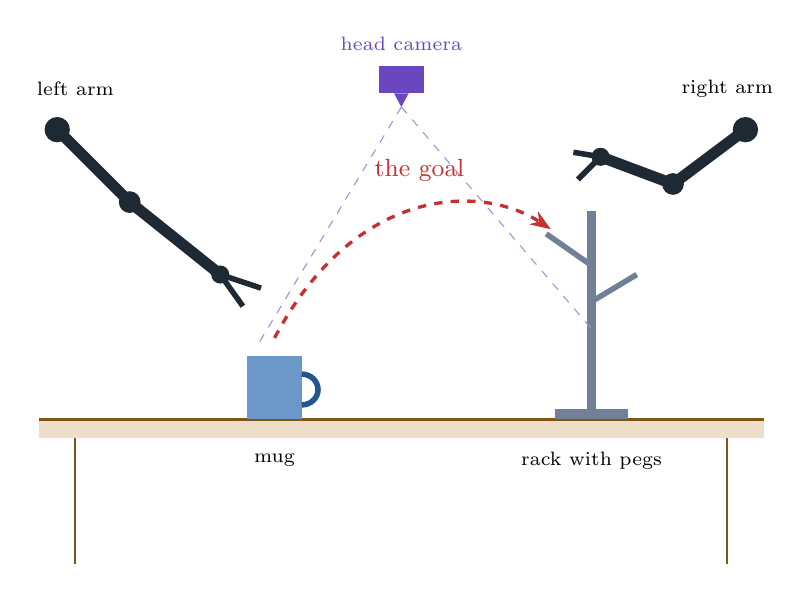
\begin{tikzpicture}[scale=1.15]
  \robotscene
  \draw[rose,very thick,->,dashed] (-1.4,0.9) .. controls (-0.5,2.6) and (0.9,2.6) .. (1.65,2.1);
  \node[font=\small,text=rose] at (0.2,2.75) {the goal};
\end{tikzpicture}
\vspace{1.0cm}

\begin{tcolorbox}[enhanced,colback=skylight,colframe=sky,arc=3mm,width=0.86\textwidth,boxrule=0.8pt]
\centering\small
This guide explains the project from zero: what the robot does, who the ``team'' inside the
software is, how one episode runs, how the code is organised, how to change things, and how to
set it up and run it, on your own computer or on rented cloud GPUs (Modal). New in 1.1: the
three big pieces and where Opus comes in (Section~\ref{sec:pieces}), the development ladder
(Section~\ref{sec:ladder}) and running on Modal. Coloured boxes help you find your way:\\[6pt]
\colorbox{sunlight}{\faChild\ simple explanation}\quad
\colorbox{skylight}{\faLightbulb\ key idea}\quad
\colorbox{leaflight}{\faWrench\ where to change it}\quad
\colorbox{roselight}{\faExclamationTriangle\ careful}
\end{tcolorbox}
\vfill
{\small\color{stone} Covers branch \texttt{modal-simulator}. File and line references point to that code.}
\end{titlepage}

{\small\tableofcontents}
\newpage

% ================================================================ 1
\section{The story in one page}

\begin{eli5}
There is a robot with \textbf{two arms} standing at a table. On the table there is a \textbf{mug}.
Next to it stands a little tree-shaped \textbf{rack} with pegs sticking out. The robot's job is to
pick up the mug and \textbf{hang it on a peg by its handle}.

The robot already learned how to do this by \emph{watching lots of examples}, a bit like a child
copying a grown-up. That learned skill is called the \textbf{policy}. It is good at most of the
job but often gets wobbly at the very end, when the handle has to slide onto the peg.

We are \textbf{not} allowed to teach the robot again. Instead, we add a \textbf{coach} who watches
through the robot's cameras every few moments and says ``keep going'', ``try this careful move
instead'', or ``stop, this is not safe''. The coach can only choose from \textbf{six move cards}.
It never wiggles the robot's joints by itself.
\end{eli5}

\begin{figure}[H]
\centering
\begin{tikzpicture}[node distance=9mm and 17mm]
  \node[box=grape,minimum width=3.1cm,minimum height=1.6cm] (eyes) {\Large\faEye\\[2pt]\textbf{Eyes}\\\scriptsize cameras + depth\\\scriptsize SAM 3 masks};
  \node[box=sky,minimum width=3.1cm,minimum height=1.6cm,right=of eyes] (coach) {\Large\faBrain\\[2pt]\textbf{Coach}\\\scriptsize Claude Opus planner\\\scriptsize picks ONE move card};
  \node[box=leaf,minimum width=3.1cm,minimum height=1.6cm,right=of coach] (muscle) {\Large\faRobot\\[2pt]\textbf{Muscle memory}\\\scriptsize frozen Neotix policy\\\scriptsize (the VLA)};
  \node[box=sun,minimum width=3.1cm,minimum height=1.6cm,below=of eyes] (ref) {\Large\faClipboardList\\[2pt]\textbf{Checklist}\\\scriptsize predicates:\\\scriptsize yes / no / don't know};
  \node[box=rose,minimum width=3.1cm,minimum height=1.6cm,below=of coach] (safety) {\Large\faLock\\[2pt]\textbf{Safety officer}\\\scriptsize skill executor\\\scriptsize budgets + limits};
  \node[box=stone,minimum width=3.1cm,minimum height=1.6cm,below=of muscle] (hands) {\Large\faHandPaper\\[2pt]\textbf{Careful hands}\\\scriptsize analytic skills\\\scriptsize small exact moves};
  \draw[flow] (eyes) -- node[lbl,above]{what I see} (coach);
  \draw[flow] (coach) -- node[lbl,above]{``go on''} (muscle);
  \draw[flow] (eyes) -- node[lbl,left]{evidence} (ref);
  \draw[flow] (ref) -- node[lbl,above]{facts} (safety);
  \draw[flow] (coach) -- node[lbl,right]{move card} (safety);
  \draw[flow] (safety) -- node[lbl,above]{exact move} (hands);
  \draw[flow] (safety.north east) -- node[lbl,right,pos=0.4]{guarded} (muscle.south west);
\end{tikzpicture}
\caption{The ``team'' inside the software. Each box is a real part of the code.}
\end{figure}

\begin{keyidea}
\textbf{One move card per turn.} The coach (Opus) reads the camera pictures and a few facts, then
picks exactly one bounded skill. The software checks the card, the robot does it, and the coach
gets fresh pictures. Nothing the coach says can move a joint directly.
\end{keyidea}

\subsection*{Why is it built like this?}
\begin{itemize}
  \item \textbf{The policy is frozen.} It was trained elsewhere and is published as \nolinkurl{Neotix-Robotics/robotwin-hanging-mug-dit}. We only \emph{use} it.
  \item \textbf{Language models are bad at joint angles} but good at looking at pictures and judging ``is this going well?''. So Opus judges and chooses, and code does the exact maths.
  \item \textbf{Safety first.} Every move has hard limits (how far, how fast, how many tries). If anything is uncertain, the robot stops instead of guessing.
\end{itemize}

% ================================================================ 2
\section{Words you will see}

\begin{center}
\small
\begin{tabularx}{\textwidth}{>{\leavevmode\bfseries\color{sky}}p{3.3cm}X}
\toprule
Word & Plain meaning \\
\midrule
Joint & A robot ``elbow'' that can bend. Each arm has six. \\
Gripper & The robot's two-finger hand. \code{0} = closed, \code{1} = open. \\
TCP / end effector & The point between the fingers. Moves are described by where this point goes. \\
14-DoF & 14 numbers that control both arms: 6 joints + 1 gripper per arm. \\
Policy / VLA & ``Vision-Language-Action'' model: pictures in, robot actions out. Ours is \emph{frozen}. \\
Chunk & The policy answers with a short list of actions (e.g.\ 8) at once. \\
Simulator & A video-game-like world (RoboTwin) with real physics, so nothing breaks. \\
Episode / seed & One attempt at the task. The seed decides where the mug starts. \\
Observation & One snapshot: 3 camera pictures + the 14 numbers. Each has a sequence number. \\
RGB-D & Colour picture (RGB) plus Depth: how far away each pixel is. \\
Calibration & The camera's ``lens settings'' (intrinsic) and position (extrinsic). Needed to turn pixels into 3D points. \\
Mask / SAM 3 & A cut-out showing which pixels are the mug, rack or table. SAM 3 makes them. \\
Planner & The coach. Either Claude Opus or a fixed script. \\
Skill & One of the six move cards (Section~\ref{sec:skills}). \\
Predicate & A checklist question like ``is the mug lifted?'' Answer: \code{true}, \code{false} or \code{null} (unknown). \\
Anchor & A named 3D target such as \code{mug_pregrasp} or \code{rack_seat}, freshly computed each time. \\
Oracle & ``Cheating'' simulator knowledge (exact mug position). Only for debugging, never shown to the coach. \\
Harness & Our code around the frozen policy: the coach, the checklist, the move cards and the safety rules. \\
RoboTwin & The simulator task suite. Our task is \code{hanging_mug}. \\
SAPIEN & The physics engine and picture-drawing (rendering) engine under RoboTwin. \\
CuRobo & A GPU motion planner: turns ``put the hand there'' into a safe joint path. \\
Vulkan & The graphics driver language SAPIEN uses to draw pictures on an NVIDIA GPU. \\
Modal & A cloud service that rents GPUs by the second. Runs the policy, SAM 3 and, optionally, whole episodes. \\
Container & A fresh, clean rented computer that Modal starts for one job and throws away afterwards. \\
Volume & A cloud folder on Modal that keeps files between containers (assets, run results). \\
Secret & A password (API key or token) stored on Modal, never written in the code. \\
\bottomrule
\end{tabularx}
\end{center}

% ================================================================ 3 (new)
\section{The three big pieces}
\label{sec:pieces}

\begin{eli5}
Think of a \textbf{puppet show}. The \textbf{stage} is the simulator: a pretend world where the
table, the mug, the rack and the robot live, and where things fall and bump like in real life.
The \textbf{team behind the stage} is the harness: our own code, which decides what the robot may
do next and makes sure it is safe. Some team members are so big that they live far away on
\textbf{rented computers in the cloud}: the policy (muscle memory), SAM~3 (the eyes that cut out
objects) and Opus (the coach who talks).
\end{eli5}

\begin{figure}[H]
\centering
\begin{tikzpicture}[every node/.style={font=\small}]
  \node[box=sun,minimum width=3.8cm,minimum height=2.6cm,text width=3.5cm] (stage) at (0,0)
    {\Large\faTheaterMasks\\[2pt]\textbf{1. The stage}\\\scriptsize simulator\\\scriptsize RoboTwin + SAPIEN + CuRobo};
  \node[box=sky,minimum width=3.8cm,minimum height=2.6cm,text width=3.5cm] (team) at (5.6,0)
    {\Large\faUsers\\[2pt]\textbf{2. The team}\\\scriptsize the harness (our code)\\\scriptsize \code{harness/}, \code{run_skills.py}};
  \node[box=leaf,minimum width=3.8cm,minimum height=2.6cm,text width=3.5cm] (cloud) at (11.2,0)
    {\Large\faCloud\\[2pt]\textbf{3. Cloud helpers}\\\scriptsize policy + SAM 3 on Modal\\\scriptsize Opus on Anthropic};
  \draw[<->,thick] (stage) -- node[lbl,above]{pictures,}node[lbl,below]{moves} (team);
  \draw[<->,thick,dashed] (team) -- node[lbl,above]{questions,}node[lbl,below]{answers} (cloud);
\end{tikzpicture}
\caption{The whole project is these three pieces talking to each other.}
\end{figure}

\subsection{Piece 1: the simulator (the stage)}

\begin{eli5}
The simulator is a \textbf{video game with real physics}. Nothing breaks, nothing costs money if it
falls, and you can start again with a fresh table. The \textbf{seed} is like the dice roll that
decides where the mug starts. Seed 3 always gives the same starting table.
\end{eli5}

It is made of layers, like a cake:

\begin{figure}[H]
\centering
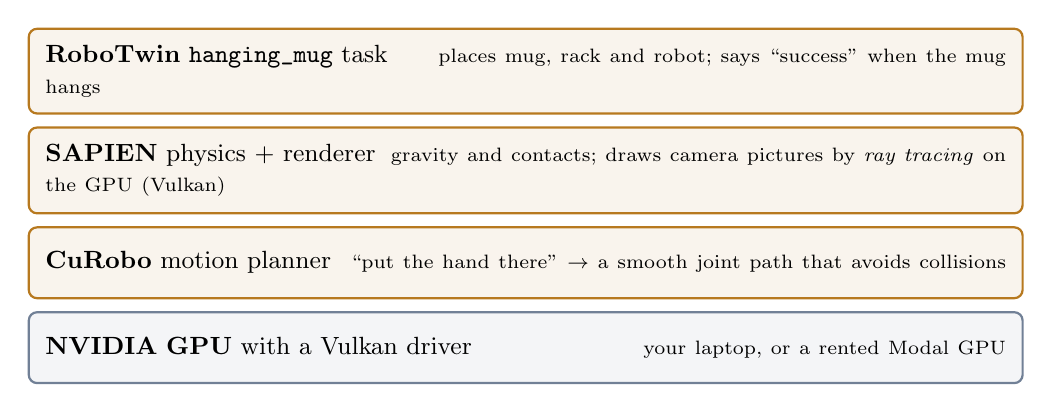
\begin{tikzpicture}[every node/.style={font=\small},
    layer/.style={box=#1,minimum width=12.6cm,minimum height=0.9cm,text width=12.2cm,align=left}]
  \node[layer=sun] (l1) at (0,0) {\textbf{RoboTwin} \code{hanging_mug} task \hfill \scriptsize places mug, rack and robot; says ``success'' when the mug hangs};
  \node[layer=sun,below=1.5mm of l1] (l2) {\textbf{SAPIEN} physics + renderer \hfill \scriptsize gravity and contacts; draws camera pictures by \emph{ray tracing} on the GPU (Vulkan)};
  \node[layer=sun,below=1.5mm of l2] (l3) {\textbf{CuRobo} motion planner \hfill \scriptsize ``put the hand there'' $\rightarrow$ a smooth joint path that avoids collisions};
  \node[layer=stone,below=1.5mm of l3] (l4) {\textbf{NVIDIA GPU} with a Vulkan driver \hfill \scriptsize your laptop, or a rented Modal GPU};
\end{tikzpicture}
\caption{The simulator stack. The pinned versions are in the README; our renderer tweak is \code{patches/robotwin-renderer.patch}.}
\end{figure}

Our code talks to the simulator through three small files:
\begin{itemize}
  \item \code{harness/environment/robotwin.py} builds the task (\code{build_task}) and packs one
        observation: three pictures, optional depth, the 14 numbers and the success flag (\code{observation_of}).
  \item \code{development/simulator/local_simulator.py} (\code{LocalSimulator}) owns \textbf{one}
        RoboTwin task in this process: reset with a seed, then step.
  \item \code{harness/environment/local.py} (\code{LocalEnvironmentClient}) is what the skills use:
        \code{observe}, \code{step}, and for careful moves \code{plan} (CuRobo) and \code{tick} (one physics step).
\end{itemize}

\begin{keyidea}
\textbf{Pictures are the slow part.} We measured each piece (Section~\ref{sec:speed}): one physics
step takes about 0.1\,ms, a CuRobo plan about 0.3\,s, but \textbf{drawing three camera pictures
with depth takes about 0.8\,s} on a laptop GPU. An episode draws hundreds of pictures, so a faster
GPU (for example on Modal) helps the most.
\end{keyidea}

\begin{careful}
RoboTwin changes the program's working folder when it starts, so run \textbf{one simulator per
process}. Its renderer needs a working NVIDIA Vulkan driver; on laptops with two GPUs, tell Vulkan
to use only NVIDIA (Section~\ref{sec:trouble}).
\end{careful}

\subsection{Piece 2: the harness (the team)}

\begin{eli5}
The harness is the \textbf{rulebook plus the team} that stands between the coach and the robot.
The coach may only hand in a move card. The team checks the card, does the exact maths, plays the
move in small safe pieces, and writes everything down. The harness never teaches the robot
anything new: the policy stays exactly as it was trained.
\end{eli5}

How it is set up today, in the order things happen:

\begin{figure}[H]
\centering
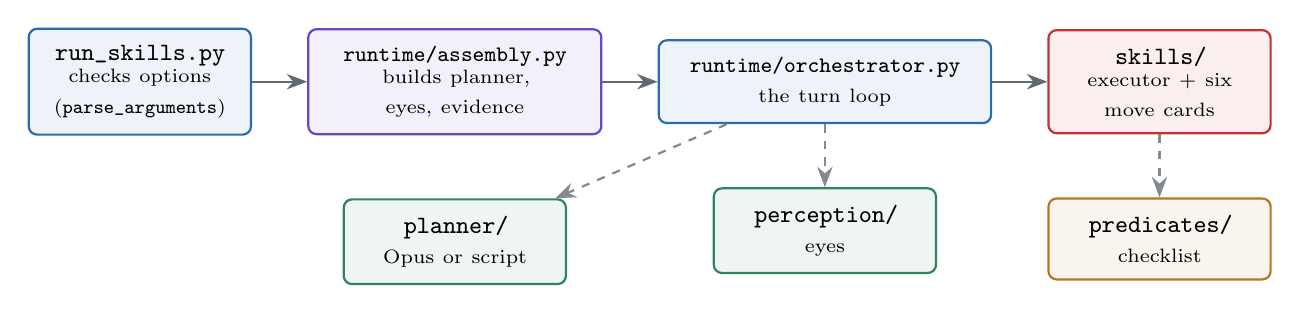
\begin{tikzpicture}[node distance=5mm and 7mm,every node/.style={font=\small}]
  \node[box=sky,text width=2.4cm] (cli) {\code{run_skills.py}\\\scriptsize checks options\\\scriptsize (\code{parse_arguments})};
  \node[box=grape,text width=3.3cm,right=of cli] (asm) {{\footnotesize\code{runtime/assembly.py}}\\\scriptsize builds planner,\\\scriptsize eyes, evidence};
  \node[box=sky,text width=3.8cm,right=of asm] (orc) {{\footnotesize\code{runtime/orchestrator.py}}\\\scriptsize the turn loop};
  \node[box=rose,text width=2.4cm,right=of orc] (exe) {\code{skills/}\\\scriptsize executor + six\\\scriptsize move cards};
  \draw[flow] (cli) -- (asm); \draw[flow] (asm) -- (orc); \draw[flow] (orc) -- (exe);
  \node[box=leaf,text width=2.4cm,below=8mm of asm] (pl) {\code{planner/}\\\scriptsize Opus or script};
  \node[box=leaf,text width=2.4cm,below=8mm of orc] (pe) {\code{perception/}\\\scriptsize eyes};
  \node[box=sun,text width=2.4cm,below=8mm of exe] (pr) {\code{predicates/}\\\scriptsize checklist};
  \draw[dflow] (orc) -- (pl); \draw[dflow] (orc) -- (pe); \draw[dflow] (exe) -- (pr);
\end{tikzpicture}
\caption{The harness in one picture. Section~\ref{sec:loop} explains the turn loop in detail.}
\end{figure}

Three switches decide \emph{where the evidence comes from}. Pick exactly one of the first two
(the third can be added to the second):

\begin{center}
\small
\begin{tabularx}{\textwidth}{>{\footnotesize\raggedright\arraybackslash}p{4.8cm}>{\raggedright\arraybackslash}X>{\raggedright\arraybackslash}p{3.2cm}}
\toprule
Evidence mode & What it means & Use it for \\
\midrule
\opt{development-oracle} & The simulator secretly tells the checklist the true mug position. Opus never sees it. & debugging skills; cheapest runs \\
\opt{perception-factory}\newline{\footnotesize\code{...modal_sam3:create_detector}} & Real ``eyes'': SAM~3 masks + depth + Opus keypoints. What a real robot could know. & honest full-task runs \\
\opt{planner-pixel-grounding} & Opus also points at pixels for targets inside its move card. & extra fallback for anchors \\
\bottomrule
\end{tabularx}
\end{center}

\subsection{Piece 3: the cloud helpers}

\begin{center}
\small
\begin{tabularx}{\textwidth}{>{\raggedright\arraybackslash}p{3.0cm}>{\raggedright\arraybackslash}p{4.1cm}>{\raggedright\arraybackslash}p{2.0cm}X}
\toprule
Helper & Code & Runs on & What it does \\
\midrule
Neotix policy & {\footnotesize\code{modal_apps/policy.py}} & Modal T4 & pictures + 14 numbers in, a chunk of actions out. Frozen. \\
SAM 3 & {\footnotesize\code{modal_apps/sam3.py}} & Modal T4 & cuts out mug, rack and table in one RGB picture. \\
Claude Opus & {\footnotesize\code{harness/planner/}\newline\code{anthropic.py}} & Anthropic API & the coach; see the next subsection. \\
Episode runner \emph{(new)} & {\footnotesize\code{modal_apps/simulator.py}} & Modal L4 & runs a \emph{whole} episode (simulator + harness) in the cloud. Optional. \\
\bottomrule
\end{tabularx}
\end{center}
Idle helpers switch themselves off (policy after 10 minutes, SAM~3 after 2), so they only cost money while used.

\subsection{Where Opus comes in}
\label{sec:opus}

\begin{eli5}
Opus is the coach who \textbf{looks and talks} but never touches the robot. It has up to five
jobs. The first is always on when you choose \opt{planner anthropic}; the others are switched on by
the config or a flag. Every job sends Opus only public pictures and facts, and every answer is
checked by code before it is used.
\end{eli5}

\begin{center}
\small
\begin{tabularx}{\textwidth}{>{\raggedright\arraybackslash}p{3.3cm}>{\raggedright\arraybackslash}p{2.1cm}>{\footnotesize\raggedright\arraybackslash}X>{\footnotesize\raggedright\arraybackslash}p{3.3cm}}
\toprule
Opus job & When & Code & Switched on by \\
\midrule
\textbf{1. Pick the next move card} & every turn & \code{AnthropicPlanner.select}\newline(\code{planner/anthropic.py}) & \opt{planner anthropic} \\
\textbf{2. Find the rack peg} (three keypoints) & once, after reset & \code{assembly.}\newline\code{initialize_rack_frame},\newline\code{perception/opus_frame.py} & \code{perception.}\newline\code{opus_rack_grounding} \\
\textbf{3. Find the mug handle} (three keypoints) & when a hang target is needed & \code{OpusObjectFrameGrounder} (\code{opus_frame.py}) & needs job 2 \\
\textbf{4. Point at the mug's bottom} for lift height & when lift is checked & \code{OpusMugSupportGrounder}\newline(\code{perception/table_plane.py}) & \code{perception.}\newline\code{opus_mug_lift_}\newline\code{grounding} \\
\textbf{5. Choose target pixels} inside its card & when a move needs a target & \code{PlannerPixelAnchorPreparer}\newline(\code{perception/preparation.py}) & \opt{planner-}\newline\texttt{pixel-grounding} \\
\bottomrule
\end{tabularx}
\end{center}

\begin{figure}[H]
\centering
\begin{tikzpicture}[node distance=4mm and 4mm,every node/.style={font=\scriptsize}]
  \node[box=sun,text width=1.6cm] (r) {reset\\seed 3};
  \node[box=grape,text width=1.9cm,right=of r] (j2) {\faBrain\ job 2\\rack peg frame};
  \node[box=grape,text width=2.0cm,right=of j2] (j4) {table plane +\\\faBrain\ job 4 ready};
  \node[box=grape,text width=2.0cm,right=10mm of j4] (j1) {\faBrain\ job 1\\pick a card\\(+ job 5 pixels)};
  \node[box=rose,text width=2.0cm,right=of j1] (ex) {executor:\\policy \faCloud\ or\\CuRobo};
  \node[box=leaf,text width=2.2cm,below=7mm of ex] (see) {\faCloud\ SAM 3 masks\\+ \faBrain\ jobs 3, 4};
  \node[box=sun,text width=2.0cm,left=of see] (chk) {checklist\\(predicates)};
  \draw[flow] (r) -- (j2); \draw[flow] (j2) -- (j4); \draw[flow] (j4) -- (j1);
  \draw[flow] (j1) -- (ex); \draw[flow] (ex) -- (see); \draw[flow] (see) -- (chk); \draw[flow] (chk) -| (j1);
  \begin{scope}[on background layer]
    \node[zone=sky,fit=(j1)(ex)(see)(chk),label={[font=\scriptsize\bfseries,text=sky]above:repeat every turn}] {};
  \end{scope}
\end{tikzpicture}
\caption{One full-task episode in time. Purple boxes are moments when Opus is asked something.}
\end{figure}

\begin{careful}
Opus calls cost money and take seconds (about 12\,s per planner turn in our runs). The config
limits them (\code{anthropic.max_calls}) and names the model explicitly (\code{claude-opus-5});
there is no fallback model. Simulator-only facts are filtered out before anything reaches Opus.
\end{careful}

% ================================================================ 3
\section{The world the robot lives in}

\subsection{The scene and the three cameras}
The simulator is \textbf{RoboTwin} running the \code{hanging_mug} task. The robot has three
cameras. Every observation contains all three pictures.

\begin{figure}[H]
\centering
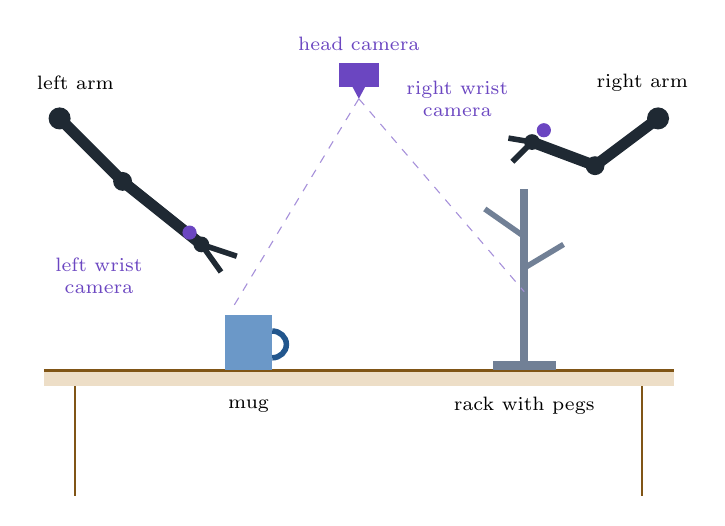
\begin{tikzpicture}[scale=1.0]
  \robotscene
  % wrist cameras
  \fill[grape] (-2.15,1.75) circle (0.09);
  \fill[grape] (2.35,3.05) circle (0.09);
  \node[font=\scriptsize,text=grape,align=center] at (-3.3,1.2) {left wrist\\camera};
  \node[font=\scriptsize,text=grape,align=center] at (1.25,3.45) {right wrist\\camera};
\end{tikzpicture}
\caption{The scene. Camera names in the code: \code{head_camera}, \code{left_camera}, \code{right_camera}.}
\end{figure}

\subsection{Fourteen numbers drive the robot}
The policy reads the pictures plus 14 numbers, and answers with 14 new numbers per step.

\begin{figure}[H]
\centering
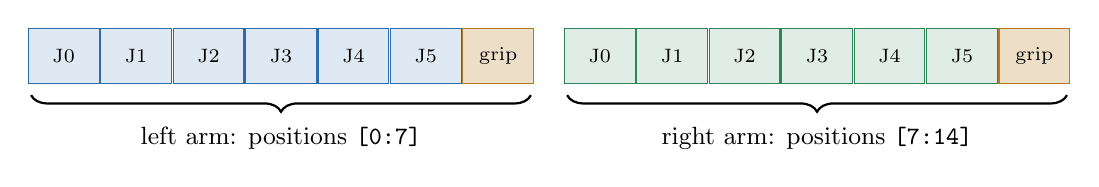
\begin{tikzpicture}[x=0.92cm]
  \foreach \i in {0,...,5} {\node[draw=sky,fill=sky!15,minimum width=0.9cm,minimum height=0.7cm,font=\scriptsize] at (\i,0) {J\i};}
  \node[draw=sun,fill=sun!25,minimum width=0.9cm,minimum height=0.7cm,font=\scriptsize] at (6,0) {grip};
  \foreach \i in {0,...,5} {\node[draw=leaf,fill=leaf!15,minimum width=0.9cm,minimum height=0.7cm,font=\scriptsize] at (\i+7.4,0) {J\i};}
  \node[draw=sun,fill=sun!25,minimum width=0.9cm,minimum height=0.7cm,font=\scriptsize] at (13.4,0) {grip};
  \draw[decorate,decoration={brace,amplitude=6pt,mirror},thick] (-0.45,-0.5) -- (6.45,-0.5) node[midway,below=8pt,font=\small] {left arm: positions \code{[0:7]}};
  \draw[decorate,decoration={brace,amplitude=6pt,mirror},thick] (6.95,-0.5) -- (13.85,-0.5) node[midway,below=8pt,font=\small] {right arm: positions \code{[7:14]}};
\end{tikzpicture}
\caption{The 14-number action layout, defined once in \code{harness/environment/layout.py}.}
\end{figure}

\subsection{Two kinds of time}
\begin{itemize}
  \item \textbf{Policy actions}: one action = one call to RoboTwin's \code{take_action}, which itself runs many physics steps. The policy sends actions in chunks.
  \item \textbf{Physics ticks}: the careful analytic skills move the arm one tick at a time. Physics runs at \textbf{250 ticks per second}, so 125 ticks is half a second.
\end{itemize}

% ================================================================ 4
\section{The task is split into three phases}

\begin{eli5}
Hanging a mug is hard to do in one go, so the robot does it in three chapters. The left hand picks
up the mug. Then it puts it back down nearby so the right hand can take it. Then the right hand
picks it up and hangs it on the rack. You can only go forward to the next chapter, never back.
\end{eli5}

\begin{figure}[H]
\centering
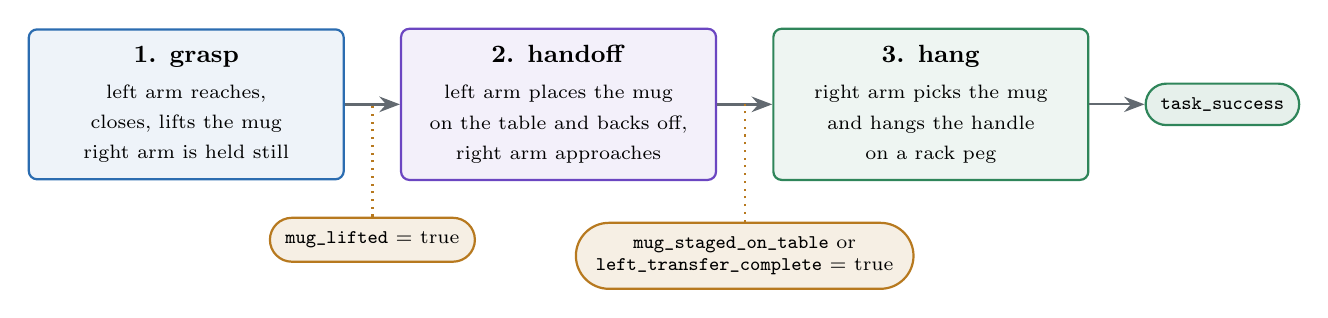
\begin{tikzpicture}[node distance=4mm and 7mm]
  \node[box=sky,minimum width=4cm,minimum height=1.9cm] (g) {\textbf{1. grasp}\\[2pt]\scriptsize left arm reaches,\\\scriptsize closes, lifts the mug\\\scriptsize right arm is held still};
  \node[box=grape,minimum width=4cm,minimum height=1.9cm,right=of g] (h) {\textbf{2. handoff}\\[2pt]\scriptsize left arm places the mug\\\scriptsize on the table and backs off,\\\scriptsize right arm approaches};
  \node[box=leaf,minimum width=4cm,minimum height=1.9cm,right=of h] (k) {\textbf{3. hang}\\[2pt]\scriptsize right arm picks the mug\\\scriptsize and hangs the handle\\\scriptsize on a rack peg};
  \draw[flow,line width=1.3pt] (g) -- (h);
  \draw[flow,line width=1.3pt] (h) -- (k);
  \node[pill=sun,font=\scriptsize] (m1) at ($(g.south)!0.5!(h.south)+(0,-0.75)$) {\code{mug_lifted} = true};
  \node[pill=sun,font=\scriptsize,align=center] (m2) at ($(h.south)!0.5!(k.south)+(0,-0.95)$) {\code{mug_staged_on_table} or\\\code{left_transfer_complete} = true};
  \draw[sun,thick,dotted] (m1.north) -- ($(g.east)!0.5!(h.west)$);
  \draw[sun,thick,dotted] (m2.north) -- ($(h.east)!0.5!(k.west)$);
  \node[pill=leaf,right=7mm of k,font=\scriptsize] (ts) {\code{task_success}};
  \draw[flow] (k) -- (ts);
\end{tikzpicture}
\caption{Phases and the public milestones that unlock the next phase.}
\end{figure}

\begin{keyidea}
A \textbf{true public milestone} sets the minimum phase. When the cameras cannot tell (the
answer is \code{null}), Opus may move the phase forward by its own visual judgement, but only
\textbf{one step per turn}. The hang phase additionally needs the staged-mug milestone.
See \srcref{harness/planner/anthropic.py:294} (\code{_public_phase_floor}) and \code{_resolve_phase}.
\end{keyidea}

% ================================================================ 5
\section{One turn of the loop}
\label{sec:loop}

Every episode is a loop of \textbf{turns}. One turn = look, decide, check, do, record.

\begin{figure}[H]
\centering
\begin{tikzpicture}
  \def\R{3.3}
  \node[box=grape,minimum width=2.9cm] (a) at (90:\R) {\faCamera\ \textbf{1. Observe}\\\scriptsize 3 pictures + 14 numbers};
  \node[box=sun,minimum width=2.9cm] (b) at (30:\R) {\faClipboardList\ \textbf{2. Checklist}\\\scriptsize evaluate predicates};
  \node[box=sky,minimum width=2.9cm] (c) at (-30:\R) {\faBrain\ \textbf{3. Decide}\\\scriptsize planner picks 1 skill};
  \node[box=stone,minimum width=2.9cm] (d) at (-90:\R) {\faCogs\ \textbf{4. Prepare}\\\scriptsize refresh 3D anchor};
  \node[box=rose,minimum width=2.9cm] (e) at (-150:\R) {\faRobot\ \textbf{5. Execute}\\\scriptsize guarded skill run};
  \node[box=leaf,minimum width=2.9cm] (f) at (150:\R) {\faFolder\ \textbf{6. Record}\\\scriptsize logs + fresh state};
  \draw[flow] (a) to[bend left=15] (b);
  \draw[flow] (b) to[bend left=15] (c);
  \draw[flow] (c) to[bend left=15] (d);
  \draw[flow] (d) to[bend left=15] (e);
  \draw[flow] (e) to[bend left=15] (f);
  \draw[flow] (f) to[bend left=15] (a);
  \node[align=center,font=\small] at (0,0) {\textbf{one turn}\\[2pt]\scriptsize repeat until\\\scriptsize success, abort\\\scriptsize or budget ends};
\end{tikzpicture}
\caption{The turn loop, implemented in \code{SkillOrchestrator.run} (\srcref{harness/runtime/orchestrator.py:219}).}
\end{figure}

\subsection{What happens after a skill finishes?}

\begin{figure}[H]
\centering
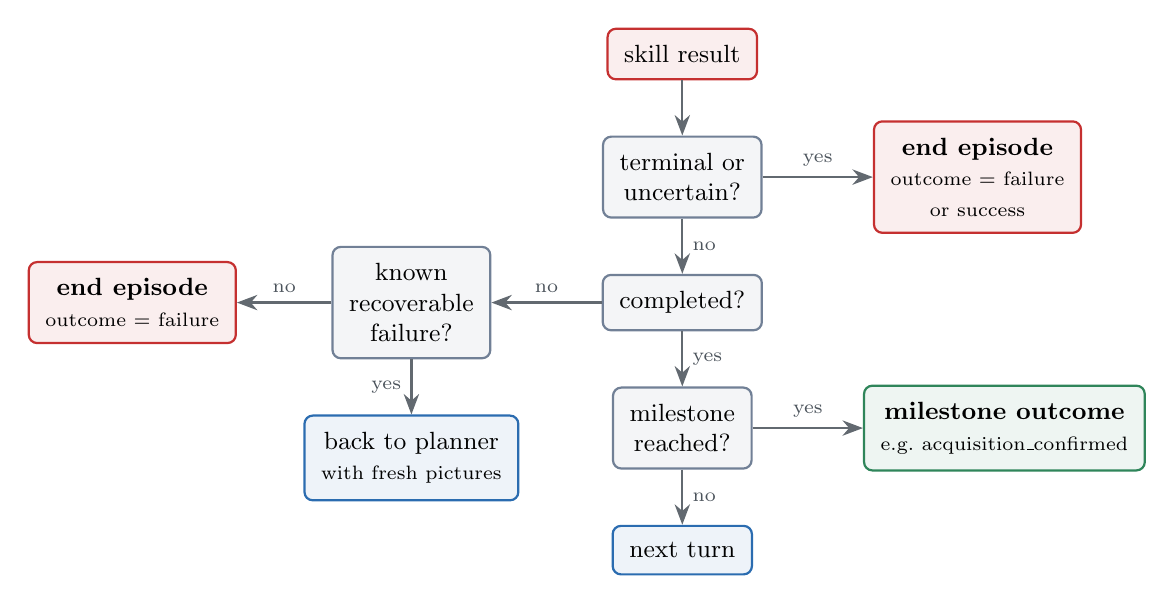
\begin{tikzpicture}[node distance=7mm and 9mm]
  \node[box=rose] (res) {skill result};
  \node[box=stone,below=of res] (q1) {terminal or\\uncertain?};
  \node[box=rose,right=14mm of q1] (stop) {\textbf{end episode}\\\scriptsize outcome = failure\\\scriptsize or success};
  \node[box=stone,below=of q1] (q2) {completed?};
  \node[box=stone,left=14mm of q2] (q3) {known\\recoverable\\failure?};
  \node[box=sky,below=of q3] (back) {back to planner\\\scriptsize with fresh pictures};
  \node[box=stone,below=of q2] (q4) {milestone\\reached?};
  \node[box=leaf,right=14mm of q4] (done) {\textbf{milestone outcome}\\\scriptsize e.g.\ acquisition\_confirmed};
  \node[box=sky,below=of q4] (next) {next turn};
  \draw[flow] (res) -- (q1);
  \draw[flow] (q1) -- node[lbl,above]{yes} (stop);
  \draw[flow] (q1) -- node[lbl,right]{no} (q2);
  \draw[flow] (q2) -- node[lbl,above]{no} (q3);
  \draw[flow] (q3) -- node[lbl,left]{yes} (back);
  \node[box=rose,left=12mm of q3] (stop2) {\textbf{end episode}\\\scriptsize outcome = failure};
  \draw[flow] (q3) -- node[lbl,above]{no} (stop2);
  \draw[flow] (q2) -- node[lbl,right]{yes} (q4);
  \draw[flow] (q4) -- node[lbl,above]{yes} (done);
  \draw[flow] (q4) -- node[lbl,right]{no} (next);
\end{tikzpicture}
\caption{Turn outcome decisions. ``Recoverable'' failures are a short, explicit list in \code{recovery_flags} (\srcref{harness/runtime/orchestrator.py:143}).}
\end{figure}

The recoverable failures are: a move that was rejected \emph{before} moving, a move that moved but
missed its target, a contact between the two arms, and a temporary perception gap. In every case
the planner sees fresh pictures; \textbf{motion is never replayed automatically}.

\subsection{Budgets: how much the robot may try}
\begin{center}
\small
\begin{tabular}{lll}
\toprule
Budget (\code{EpisodeBudget}) & Default & Meaning \\
\midrule
\code{max_skill_calls} & 100 & move cards per episode \\
\code{max_policy_actions} & 1200 & policy actions executed in total \\
\code{max_vla_chunks} & 150 & times the policy may be asked \\
\code{max_analytic_ticks} & 12000 & physics ticks for careful moves (48 s) \\
\code{max_turns} (\code{RunSettings}) & 20 & planner turns \\
\bottomrule
\end{tabular}
\end{center}
\srcref{harness/skills/schemas.py:123}. Configs usually override these.

% ================================================================ 6
\section{The six move cards (skills)}
\label{sec:skills}

\begin{center}
\small
\begin{tabularx}{\textwidth}{>{\bfseries}l>{\raggedright\arraybackslash}Xl>{\raggedright\arraybackslash}X}
\toprule
Skill & What it does & Arms & Limits \\
\midrule
\color{leaf}\code{vla_act} & Ask the frozen policy for short chunks and play them, with checks after every action. & both & $\le$32 chunks, $\le$24 actions/chunk \\
\color{sky}\code{move_to} & Move one hand to a fresh named target (or current pose) plus a small offset. & one & offset $\le$ 20\,cm \\
\color{sky}\code{rotate_wrist} & Turn one wrist around the vertical axis. & one & $\le$ 30$^\circ$ \\
\color{sky}\code{set_gripper} & Slowly open/close one hand. Opening needs permission. & one & 50--500 ticks ramp \\
\color{sky}\code{release} & Fully open one hand, only when support is proven. & one & guarded \\
\color{rose}\code{abort} & Stop the episode. No motion. & none & -- \\
\bottomrule
\end{tabularx}
\end{center}
\srcref{harness/skills/schemas.py:13}. Blue skills are \emph{analytic}: exact maths, no learning.

\subsection{How a VLA call plays a chunk}

\begin{figure}[H]
\centering
\begin{tikzpicture}[x=1.05cm]
  \node[box=grape,anchor=east] (pic) at (-0.4,0) {\faCamera\ fresh\\observation};
  \node[box=leaf] (pol) at (1.3,1.6) {\faCloud\ policy on Modal};
  \draw[flow] (pic.north) |- (pol.west);
  \draw[flow] (pol.east) -| node[lbl,above,pos=0.25] {8 actions} (4.5,0.35);
  \foreach \i in {1,...,8} {
    \ifnum\i<6 \def\c{leaf}\else\def\c{stone}\fi
    \node[draw=\c,fill=\c!20,minimum width=0.85cm,minimum height=0.6cm,font=\scriptsize] (act\i) at (\i+0.5,0) {a\i};
  }
  \foreach \i in {1,...,4} {\node[text=leaf,font=\scriptsize] at (\i+0.95,-0.55) {\faCheck};}
  \node[text=rose,font=\scriptsize] at (5.95,-0.55) {\faTimes};
  \draw[rose,thick,dashed] (6.0,0.6) -- (6.0,-0.75);
  \node[lbl,text=rose,above] at (6.0,0.6) {stop condition met};
  \draw[decorate,decoration={brace,amplitude=5pt,mirror},thick] (1.1,-0.8) -- (5.9,-0.8) node[midway,below=6pt,font=\scriptsize] {executed one by one, checked after each};
  \draw[decorate,decoration={brace,amplitude=5pt,mirror},thick,stone] (6.1,-0.8) -- (8.9,-0.8) node[midway,below=6pt,font=\scriptsize,text=stone] {stale tail discarded};
\end{tikzpicture}
\caption{One chunk. After every action the code checks the stop predicate, arm-to-arm contact and
the task checker. Unused actions are thrown away, never executed later (\srcref{harness/skills/vla_act.py:159}).}
\end{figure}

\begin{keyidea}
\textbf{Feedback boundary.} In Opus mode each \code{vla_act} call ends after
\code{planner_feedback_chunks} chunks (normally 1). The coach then sees new pictures and decides
again. When RoboTwin's checker first reports success, the policy may finish a fixed 16-action
follow-through so the gripper can let go cleanly (\code{NATIVE_SUCCESS_FOLLOW_THROUGH_ACTIONS}).
\end{keyidea}

\subsection{How a careful (analytic) move works}

\begin{figure}[H]
\centering
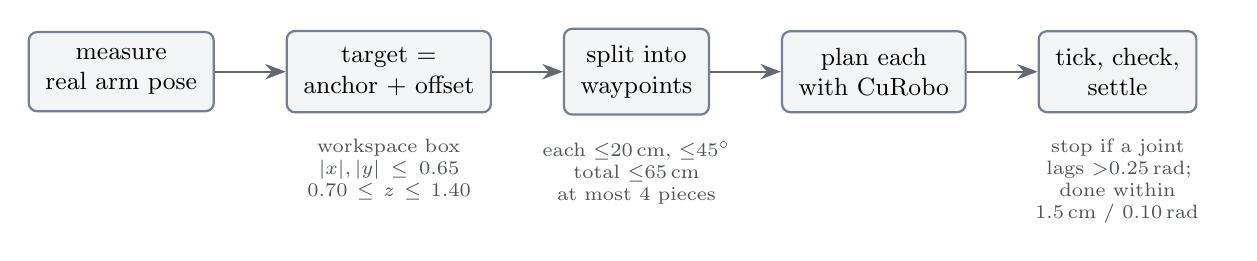
\begin{tikzpicture}[node distance=5mm and 9mm]
  \node[box=stone] (s) {measure\\real arm pose};
  \node[box=stone,right=of s] (t) {target =\\anchor + offset};
  \node[box=stone,right=of t] (w) {split into\\waypoints};
  \node[box=stone,right=of w] (p) {plan each\\with CuRobo};
  \node[box=stone,right=of p] (x) {tick, check,\\settle};
  \draw[flow] (s) -- (t); \draw[flow] (t) -- (w); \draw[flow] (w) -- (p); \draw[flow] (p) -- (x);
  \node[lbl,below=2mm of t,text width=2.6cm] {workspace box\\$|x|,|y|\le0.65$\\$0.70\le z\le1.40$};
  \node[lbl,below=2mm of w,text width=2.6cm] {each $\le$20\,cm, $\le$45$^\circ$\\total $\le$65\,cm\\at most 4 pieces};
  \node[lbl,below=2mm of x,text width=2.6cm] {stop if a joint lags $>$0.25\,rad;\\done within\\1.5\,cm / 0.10\,rad};
\end{tikzpicture}
\caption{Analytic skills always start from the \emph{measured} pose, never a remembered one (\srcref{harness/skills/analytic.py}).}
\end{figure}

% ================================================================ 7
\section{House rules that keep things safe}

\subsection{Three answers, not two}
\begin{figure}[H]
\centering
\begin{tikzpicture}[node distance=10mm]
  \node[circle,draw=leaf,fill=leaf!25,minimum size=1.6cm,thick] (t) {\Large\faCheck};
  \node[circle,draw=rose,fill=rose!20,minimum size=1.6cm,thick,right=of t] (f) {\Large\faTimes};
  \node[circle,draw=stone,fill=stone!20,minimum size=1.6cm,thick,right=of f] (u) {\Large\faQuestion};
  \node[below=2mm of t,font=\small,align=center] {\code{true}\\proven};
  \node[below=2mm of f,font=\small,align=center] {\code{false}\\proven not};
  \node[below=2mm of u,font=\small,align=center] {\code{null}\\cannot tell};
  \node[right=8mm of u,box=rose,text width=5.4cm,align=left,font=\small] {\textbf{Unknown is never treated as yes.} A missing mask is not ``the mug is gone'' and not ``the mug is lifted''.};
\end{tikzpicture}
\caption{Predicate answers (\code{PredicateResult}, \srcref{harness/predicates/base.py}).}
\end{figure}

\subsection{The wall between public and private knowledge}
\begin{figure}[H]
\centering
\begin{tikzpicture}
  \node[zone=leaf,minimum width=7.6cm,minimum height=4.5cm,label={[font=\small\bfseries,text=leaf]above:Public (what a real robot could know)}] (pub) at (0,0) {};
  \node[zone=rose,minimum width=5.0cm,minimum height=4.5cm,label={[font=\small\bfseries,text=rose]above:Private (simulator only)}] (pri) at (7.9,0) {};
  \node[box=leaf,text width=2.9cm] at (-1.8,1.25) {camera pictures};
  \node[box=leaf,text width=2.9cm] at (1.8,1.25) {depth and\\calibration};
  \node[box=leaf,text width=2.9cm] at (-1.8,0.1) {arm joint readings};
  \node[box=leaf,text width=2.9cm] at (1.8,0.1) {perception\\predicates};
  \node[box=sky] (op) at (0,-1.4) {\faBrain\ Opus sees only this side};
  \node[box=rose,text width=3.6cm] at (7.9,1.25) {exact mug pose};
  \node[box=rose,text width=3.6cm] at (7.9,0.1) {contact sensors};
  \node[box=rose,text width=3.6cm] at (7.9,-1.05) {oracle predicates\\and anchors};
  \fill[ink] (4.4,-2.3) rectangle (4.75,2.3);
  \node[rotate=90,font=\small\bfseries,text=white] at (4.575,0) {WALL};
\end{tikzpicture}
\caption{The oracle may gate execution during debugging (\opt{development-oracle}), but it is
filtered out before anything is sent to Opus (\srcref{harness/planner/prompt_builder.py}).}
\end{figure}

\subsection{Opening a hand needs proof}
The robot may only open a hand that is holding the mug when the public checklist says
that \code{release_ready} is \code{true} (the mug is resting on the table), or, at the rack,
that \code{rack_seat_aligned} is \code{true}.
The planner enforces this before anything moves:

\needspace{13\baselineskip}
\begin{lstlisting}[firstnumber=181,caption={\srcref{harness/planner/anthropic.py:181}}]
release_authorized = self._public_predicate_true(context, "release_ready")
rack_seat_authorized = (vla_phase == "hang" and
    self._public_predicate_true(context, "rack_seat_aligned"))
release_allowed = (release_authorized or
    (command.action.value == "release"
     and command.parameters.authorization == "rack_seat_alignment"
     and rack_seat_authorized))
if (not release_allowed and
        (command.action.value == "release"
         or (command.action.value == "set_gripper" and command.parameters.value > 0.0))):
    raise InvalidPlannerResponse("release_not_publicly_authorized")
\end{lstlisting}

\subsection{Other rules in one list}
\begin{itemize}
  \item \textbf{Never retry an uncertain command.} If a response is lost after sending an action, the episode stops.
  \item \textbf{Anchors expire.} A target is valid only for the observation it was computed from.
  \item \textbf{Arm contact recovery is narrow}: right hand moves 3--10\,cm away, at most 2 retreats and 3 incidents.
  \item \textbf{Grounding retries are limited}: a rejected pixel can be re-chosen at most twice, the second time from a different camera.
  \item \textbf{Logs never contain secrets} or raw provider text; only short error codes.
\end{itemize}

% ================================================================ 8
\section{The eyes: perception}

\begin{eli5}
A picture is flat. To reach for the mug, the robot needs to know \emph{where in 3D} it is. Each
camera also tells how far away every pixel is (depth). If you know which pixel is the mug and how far
away that pixel is, and where the camera is, you can work out the mug's 3D position.
\end{eli5}

\subsection{From a pixel to a 3D point}
\begin{figure}[H]
\centering
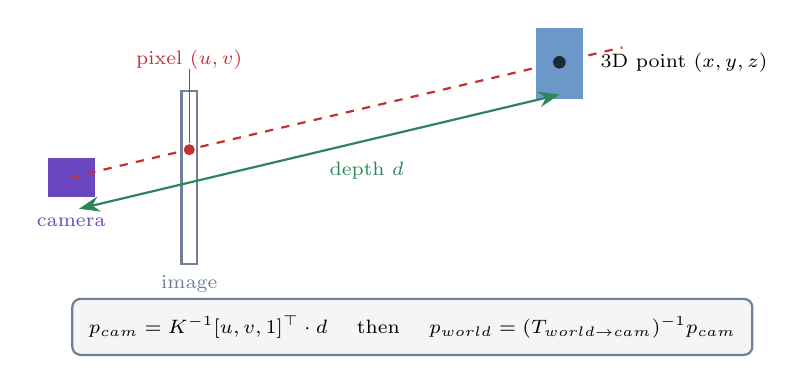
\begin{tikzpicture}
  \fill[grape] (-0.3,-0.25) rectangle (0.3,0.25);
  \node[font=\scriptsize,text=grape,below=3mm] at (0,-0.1) {camera};
  \draw[stone,thick] (1.4,-1.1) rectangle (1.6,1.1);
  \node[font=\scriptsize,text=stone] at (1.5,-1.35) {image};
  \fill[rose] (1.5,0.35) circle (0.07);
  \node[font=\scriptsize,text=rose] at (1.5,1.5) {pixel $(u,v)$};
  \draw[rose,thin] (1.5,1.38) -- (1.5,0.43);
  \draw[rose,thick,dashed] (0,0) -- (7,1.65);
  \fill[sky!70] (5.9,1.0) rectangle (6.5,1.9);
  \fill[ink] (6.2,1.46) circle (0.08);
  \node[font=\scriptsize,right] at (6.6,1.45) {3D point $(x,y,z)$};
  \draw[<->,thick,leaf] (0.1,-0.4) -- (6.2,1.05) node[midway,below right,font=\scriptsize,text=leaf] {depth $d$};
  \node[box=stone,font=\scriptsize,anchor=west] at (0,-1.9) {$p_{cam} = K^{-1}[u,v,1]^\top \cdot d$ \quad then \quad $p_{world} = (T_{world\rightarrow cam})^{-1} p_{cam}$};
\end{tikzpicture}
\caption{Unprojection. $K$ is the intrinsic matrix, $T$ the extrinsic pose.}
\end{figure}

\needspace{12\baselineskip}
\begin{lstlisting}[numbers=none,caption={\srcref{harness/perception/rgbd.py:97} \ \code{RGBDCamera.unproject} (abridged)}]
depth = self.sample_depth(u, v, radius=radius)     # local median, ignores zeros
pixel = np.array([float(u), float(v), 1.0])
camera_xyz = np.linalg.solve(self.intrinsic, pixel) * depth
camera_h = np.append(camera_xyz, 1.0)
world = np.linalg.solve(self.world_to_camera, camera_h)
return tuple(float(value) for value in world[:3] / world[3])
\end{lstlisting}

\subsection{Who looks at the pictures?}
\begin{figure}[H]
\centering
\begin{tikzpicture}[node distance=6mm and 10mm]
  \node[box=grape] (rgb) {\faCamera\ RGB picture};
  \node[box=sky,above right=2mm and 12mm of rgb] (sam) {\faCloud\ SAM 3 on Modal\\\scriptsize masks: mug, rack, table};
  \node[box=sky,below right=2mm and 12mm of rgb] (opus) {\faBrain\ Opus\\\scriptsize keypoints / support pixel};
  \node[box=leaf,right=12mm of sam] (geo) {local RGB-D geometry\\\scriptsize depth + calibration};
  \node[box=leaf,right=12mm of opus] (fr) {3D frames, anchors,\\\scriptsize lift evidence};
  \node[box=sun,right=of $(geo)!0.5!(fr)$] (pred) {predicates\\+ anchors};
  \draw[flow] (rgb) |- (sam); \draw[flow] (rgb) |- (opus);
  \draw[flow] (sam) -- (geo); \draw[flow] (opus) -- (fr); \draw[flow] (geo) -- (fr);
  \draw[flow] (geo) -| (pred); \draw[flow] (fr) -| (pred);
\end{tikzpicture}
\caption{Only RGB images leave the machine. Depth maths always stays local.}
\end{figure}

\begin{itemize}
  \item \textbf{SAM 3} (\code{harness/perception/modal_sam3.py}) draws masks. Mask confidence floors: mug 0.40, rack 0.60 (0.18 with the exploration prompt ``mug rack''), table 0.60.
  \item \textbf{Opus keypoints} (\code{opus_frame.py}) give three ordered points on the rack peg or the mug handle; three points define a little 3D coordinate frame.
  \item \textbf{Opus support pixel} (\code{table_plane.py}) marks the bottom of the mug, used to measure lift height.
\end{itemize}

\subsection{Three points make a frame}
\begin{figure}[H]
\centering
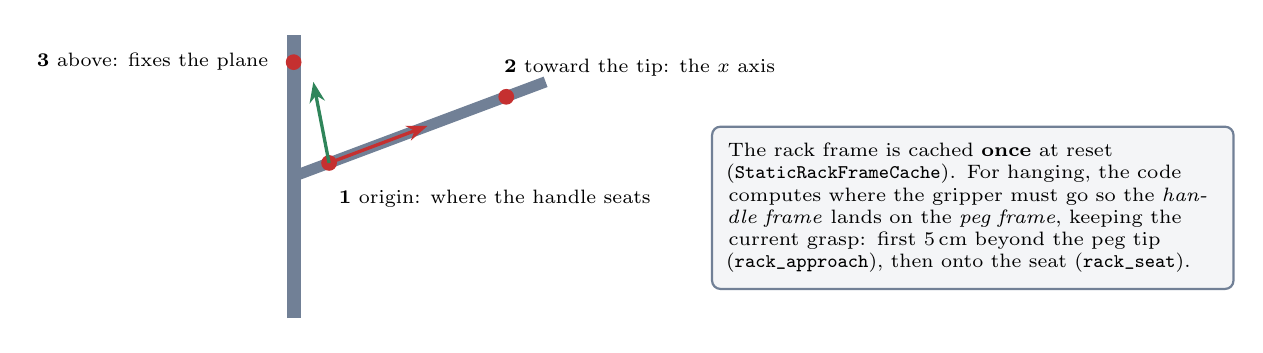
\begin{tikzpicture}
  \draw[stone,line width=5pt] (0,0) -- (0,3.6);
  \draw[stone,line width=4pt] (0,1.8) -- (3.2,3.0);
  \fill[rose] (0.45,1.97) circle (0.1);
  \node[font=\scriptsize,anchor=north west] at (0.45,1.75) {\textbf{1} origin: where the handle seats};
  \fill[rose] (2.7,2.81) circle (0.1);
  \node[font=\scriptsize,anchor=south west] at (2.55,2.95) {\textbf{2} toward the tip: the $x$ axis};
  \fill[rose] (0.0,3.25) circle (0.1);
  \node[font=\scriptsize,anchor=east] at (-0.2,3.25) {\textbf{3} above: fixes the plane};
  \draw[->,very thick,rose] (0.45,1.97) -- (1.7,2.44);
  \draw[->,very thick,leaf] (0.45,1.97) -- (0.25,3.0);
  \node[box=stone,font=\scriptsize,text width=6.2cm,align=left,anchor=west] at (5.3,1.4) {The rack frame is cached \textbf{once} at reset (\code{StaticRackFrameCache}). For hanging, the code computes where the gripper must go so the \emph{handle frame} lands on the \emph{peg frame}, keeping the current grasp: first 5\,cm beyond the peg tip (\code{rack_approach}), then onto the seat (\code{rack_seat}).};
\end{tikzpicture}
\caption{Keypoints become frames (\srcref{harness/perception/pose_grounding.py}, \code{hang_targets.py}).}
\end{figure}

\subsection{Is the mug lifted? Measuring against the table}
\begin{figure}[H]
\centering
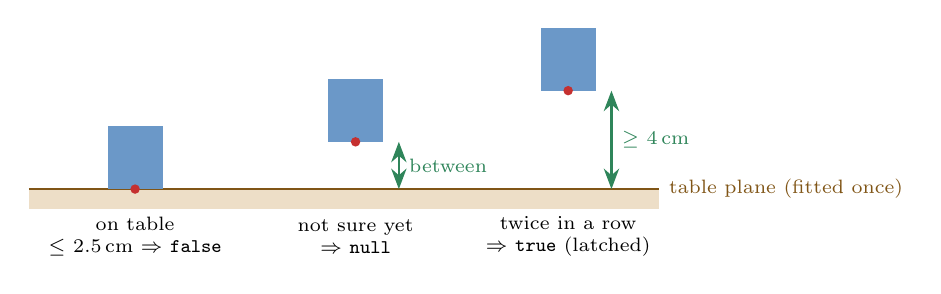
\begin{tikzpicture}
  \fill[sun!25] (0,0) rectangle (8,0.25);
  \draw[sun!70!black,thick] (0,0.25) -- (8,0.25) node[right,font=\scriptsize] {table plane (fitted once)};
  \fill[sky!70] (1,0.25) rectangle (1.7,1.05);
  \fill[rose] (1.35,0.25) circle (0.06);
  \node[font=\scriptsize,align=center] at (1.35,-0.35) {on table\\$\le$ 2.5\,cm $\Rightarrow$ \code{false}};
  \fill[sky!70] (3.8,0.85) rectangle (4.5,1.65);
  \fill[rose] (4.15,0.85) circle (0.06);
  \draw[<->,leaf,thick] (4.7,0.25) -- (4.7,0.85) node[midway,right,font=\scriptsize] {between};
  \node[font=\scriptsize,align=center] at (4.15,-0.35) {not sure yet\\$\Rightarrow$ \code{null}};
  \fill[sky!70] (6.5,1.5) rectangle (7.2,2.3);
  \fill[rose] (6.85,1.5) circle (0.06);
  \draw[<->,leaf,thick] (7.4,0.25) -- (7.4,1.5) node[midway,right,font=\scriptsize] {$\ge$ 4\,cm};
  \node[font=\scriptsize,align=center] at (6.85,-0.35) {twice in a row\\$\Rightarrow$ \code{true} (latched)};
\end{tikzpicture}
\caption{Table-relative lift evidence (\code{MugLiftEvidenceTracker}, \srcref{harness/perception/table_plane.py:196}).}
\end{figure}

\begin{changeit}
Lift thresholds are constructor arguments: \code{lifted_distance_m=0.04},
\code{table_distance_m=0.025}, \code{consecutive_observations=2} in
\code{harness/perception/table_plane.py}. Mask confidence floors are
\code{MUG_MASK_MIN_CONFIDENCE} and \code{EXPLORE_RACK_MASK_MIN_CONFIDENCE} in
\code{harness/runtime/assembly.py}. Prompts for Opus perception live in \code{harness/prompts/}.
\end{changeit}

\subsection{When a chosen pixel is bad}
\begin{figure}[H]
\centering
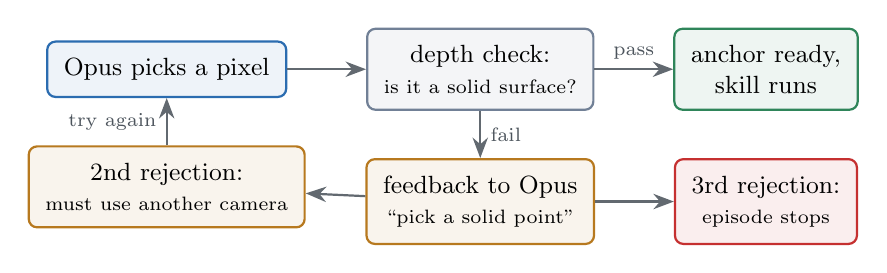
\begin{tikzpicture}[node distance=6mm and 10mm]
  \node[box=sky] (p) {Opus picks a pixel};
  \node[box=stone,right=of p] (c) {depth check:\\\scriptsize is it a solid surface?};
  \node[box=leaf,right=of c] (ok) {anchor ready,\\skill runs};
  \node[box=sun,below=of c] (fb) {feedback to Opus\\\scriptsize ``pick a solid point''};
  \node[box=sun,below=of p] (cam) {2nd rejection:\\\scriptsize must use another camera};
  \node[box=rose,right=of fb] (ab) {3rd rejection:\\\scriptsize episode stops};
  \draw[flow] (p) -- (c); \draw[flow] (c) -- node[lbl,above]{pass} (ok);
  \draw[flow] (c) -- node[lbl,right]{fail} (fb);
  \draw[flow] (fb) -- (cam); \draw[flow] (cam.north) -- node[lbl,left]{try again} (cam.north |- p.south);
  \draw[flow] (fb) -- (ab);
\end{tikzpicture}
\caption{Grounding reselection (\code{MAX_GROUNDING_RESELECTIONS = 2}, \srcref{harness/runtime/orchestrator.py:19}).}
\end{figure}

% ================================================================ 9
\section{Architecture: what runs where}

\begin{figure}[H]
\centering
\begin{tikzpicture}[scale=0.92,transform shape,every node/.style={font=\small}]
  \node[box=sky,minimum width=3.3cm] (cli) at (0,3.0) {\code{run_skills.py}\\\scriptsize CLI, one episode};
  \node[box=sky,minimum width=3.3cm] (orc) at (0,1.5) {SkillOrchestrator\\\scriptsize turn loop};
  \node[box=sky,minimum width=2.9cm] (per) at (-1.9,0) {Perception\\\scriptsize RGB-D grounding};
  \node[box=sky,minimum width=2.9cm] (exe) at (1.9,0) {SkillExecutor\\\scriptsize 6 skills + budgets};
  \node[box=sun,minimum width=2.9cm] (pred) at (-1.9,-1.5) {Predicates\\\scriptsize checklist};
  \node[box=sun,minimum width=2.9cm] (sim) at (1.9,-1.5) {RoboTwin + CuRobo\\\scriptsize physics, planning};
  \begin{scope}[on background layer]
    \node[zone=sky,fit=(cli)(per)(exe)(pred)(sim),label={[font=\small\bfseries,text=sky]above:\faLaptop\ Your machine \emph{or} a Modal episode container}] {};
  \end{scope}
  \node[box=leaf,minimum width=3.0cm] (sam) at (-7.0,0) {SAM 3\\\scriptsize \code{modal_apps/sam3.py}\\\scriptsize T4 GPU};
  \node[box=leaf,minimum width=3.0cm] (pol) at (7.0,0) {Neotix policy\\\scriptsize \code{modal_apps/policy.py}\\\scriptsize T4 GPU};
  \node[box=grape,minimum width=3.0cm] (ant) at (7.0,2.6) {Claude Opus\\\scriptsize Anthropic API};
  \begin{scope}[on background layer]
    \node[zone=leaf,fit=(sam),label={[font=\small\bfseries,text=leaf]above:\faCloud\ Modal}] {};
    \node[zone=leaf,fit=(pol),label={[font=\small\bfseries,text=leaf]below:\faCloud\ Modal}] {};
  \end{scope}
  \draw[flow] (cli) -- (orc);
  \draw[flow] (orc) -- (per); \draw[flow] (orc) -- (exe);
  \draw[flow] (per) -- (pred); \draw[flow] (exe) -- (sim);
  \draw[dflow] (orc.east) -- node[lbl,above,sloped]{pictures + facts} (ant.west);
  \draw[dflow] (exe.east) -- node[lbl,above,font=\tiny]{RGB +\\state} (pol.west);
  \draw[dflow] (per.west) -- node[lbl,above,font=\tiny]{RGB\\only} (sam.east);
\end{tikzpicture}
\caption{System architecture. Dashed arrows cross the network. The blue box runs either on your
own GPU or, unchanged, inside a Modal container (Section~\ref{sec:runmodal}).}
\end{figure}

\subsection{How the code layers depend on each other}
\begin{figure}[H]
\centering
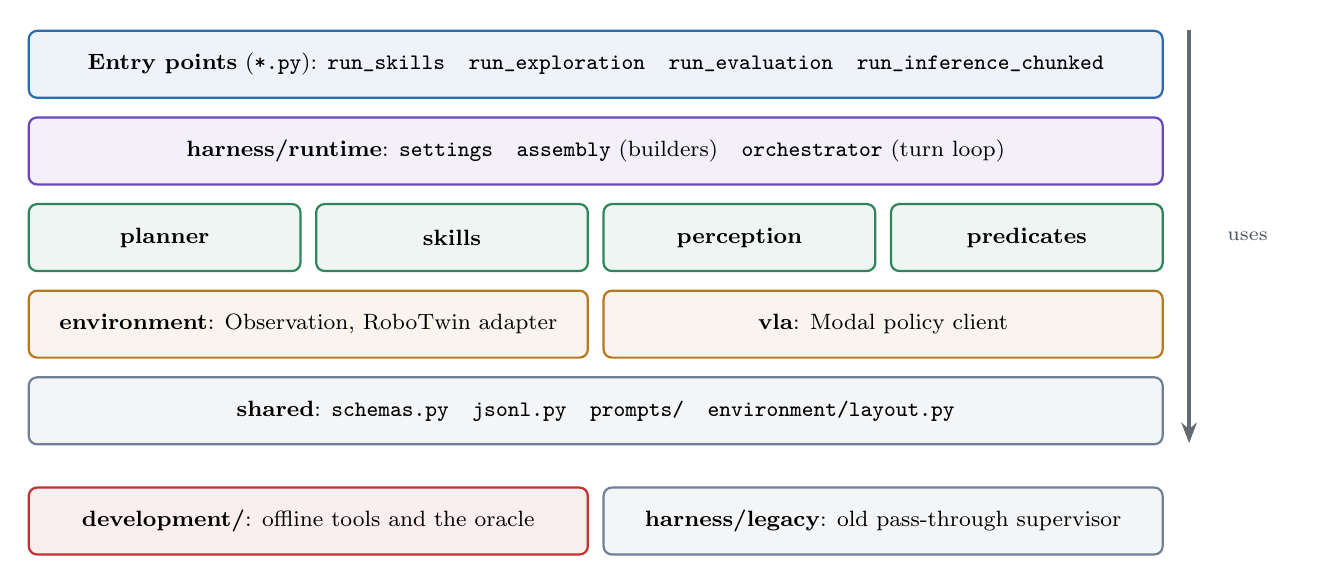
\begin{tikzpicture}[every node/.style={font=\small},
    layer/.style={box=#1,font=\footnotesize,anchor=north west,minimum height=0.85cm,inner sep=3pt}]
  \node[layer=sky,minimum width=14.4cm] at (0,0) {\textbf{Entry points} (\code{*.py}): \code{run_skills}\quad\code{run_exploration}\quad\code{run_evaluation}\quad\code{run_inference_chunked}};
  \node[layer=grape,minimum width=14.4cm] at (0,-1.1) {\textbf{harness/runtime}: \code{settings}\quad\code{assembly} (builders)\quad\code{orchestrator} (turn loop)};
  \node[layer=leaf,minimum width=3.45cm] at (0,-2.2) {\textbf{planner}};
  \node[layer=leaf,minimum width=3.45cm] at (3.65,-2.2) {\textbf{skills}};
  \node[layer=leaf,minimum width=3.45cm] at (7.3,-2.2) {\textbf{perception}};
  \node[layer=leaf,minimum width=3.45cm] at (10.95,-2.2) {\textbf{predicates}};
  \node[layer=sun,minimum width=7.1cm] at (0,-3.3) {\textbf{environment}: Observation, RoboTwin adapter};
  \node[layer=sun,minimum width=7.1cm] at (7.3,-3.3) {\textbf{vla}: Modal policy client};
  \node[layer=stone,minimum width=14.4cm] at (0,-4.4) {\textbf{shared}: \code{schemas.py}\quad\code{jsonl.py}\quad\code{prompts/}\quad\code{environment/layout.py}};
  \node[layer=rose,minimum width=7.1cm] at (0,-5.8) {\textbf{development/}: offline tools and the oracle};
  \node[layer=stone,minimum width=7.1cm] at (7.3,-5.8) {\textbf{harness/legacy}: old pass-through supervisor};
  \draw[flow,line width=1.5pt] (14.75,0) -- node[lbl,right,text width=1.2cm]{uses} (14.75,-5.25);
\end{tikzpicture}
\caption{Higher layers use lower layers, never the other way round. \code{development/} is used only by the CLIs and tests.}
\end{figure}

% ================================================================ 10
\section{Where everything lives}

\begin{figure}[H]
\centering
\begin{forest}
  for tree={font=\ttfamily\footnotesize,grow'=0,child anchor=west,parent anchor=south,anchor=west,inner ysep=1.5pt,s sep=1pt,
    calign=first,edge path={\noexpand\path [draw, \forestoption{edge}] (!u.south west) +(7.5pt,0) |- node[fill,inner sep=1.25pt] {} (.child anchor)\forestoption{edge label};},
    before typesetting nodes={if n=1{insert before={[,phantom]}}{}},fit=band,before computing xy={l=15pt}}
  [Agent-Aware-Vision-Language-Action-Model/
    [run\_skills.py \quad{\rmfamily\color{stone} one supervised episode}]
    [run\_exploration.py \quad{\rmfamily\color{stone} many episodes, one process each}]
    [run\_evaluation.py \quad{\rmfamily\color{stone} frozen, fair evaluation}]
    [run\_inference\_chunked.py \quad{\rmfamily\color{stone} baseline: policy alone}]
    [harness/
      [runtime/ \quad{\rmfamily\color{stone} settings, builders, turn loop}]
      [planner/ \quad{\rmfamily\color{stone} Opus + scripted coaches, prompt, parser}]
      [skills/ \quad{\rmfamily\color{stone} the six move cards}]
      [perception/ \quad{\rmfamily\color{stone} eyes: masks, depth, frames}]
      [predicates/ \quad{\rmfamily\color{stone} the checklist}]
      [environment/ \quad{\rmfamily\color{stone} observation, RoboTwin adapter}]
      [vla/ \quad{\rmfamily\color{stone} talk to the policy on Modal}]
      [memory/ \ exploration/ \ evaluation/]
      [prompts/ \quad{\rmfamily\color{stone} text sent to Opus}]
      [legacy/ \quad{\rmfamily\color{stone} old pass-through supervisor}]]
    [modal\_apps/
      [policy.py \ sam3.py \quad{\rmfamily\color{stone} cloud helpers}]
      [simulator.py \quad{\rmfamily\color{stone} cloud image, spike, remote episodes}]
      [episode\_request.py \quad{\rmfamily\color{stone} turns CLI options into a remote run}]]
    [development/
      [simulator/ \ replays/ \ capture/]
      [checkpoints/ \ recovery/ \ demos/]]
    [configs/ \quad{\rmfamily\color{stone} YAML presets}]
    [requirements/ \ tests/ \ patches/]
  ]
\end{forest}
\caption{Repository layout. \code{RoboTwin/}, \code{data/} and \code{docs/} are local and not in git.}
\end{figure}

\subsection{Which file do I open?}
\begin{center}
\small
\begin{tabularx}{\textwidth}{>{\raggedright\arraybackslash}Xl}
\toprule
I want to understand\ldots & Open \\
\midrule
how an episode is started and cleaned up & \code{run_skills.py} \\
how the parts are built and connected & \code{harness/runtime/assembly.py} \\
the turn-by-turn loop & \code{harness/runtime/orchestrator.py} \\
how Opus is asked and checked & \code{harness/planner/anthropic.py} \\
what Opus is told & \code{harness/prompts/common.md}, \code{full_task.md} \\
what a move card may contain & \code{harness/skills/schemas.py} \\
how the policy chunk is played & \code{harness/skills/vla_act.py} \\
how careful moves are executed & \code{harness/skills/analytic.py} \\
how pictures become 3D anchors & \code{harness/perception/grounding.py}, \code{preparation.py} \\
the checklist logic & \code{harness/predicates/} \\
how RoboTwin is started & \code{harness/environment/robotwin.py} \\
the cloud model code & \code{modal_apps/policy.py}, \code{sam3.py} \\
how an episode runs on Modal & \code{modal_apps/simulator.py}, \code{episode_request.py} \\
how the simulator is wrapped & \code{development/simulator/local_simulator.py}, \code{harness/environment/local.py} \\
\bottomrule
\end{tabularx}
\end{center}

% ================================================================ 11
\section{Code tour: how it works today}

\subsection{Starting an episode}
\code{main()} checks the command-line options with \code{parse_arguments()} \emph{before} anything
expensive starts (the Modal launcher reuses the same check on your machine), then
\code{run_episode()} owns the simulator for exactly one reset:

\needspace{12\baselineskip}
\begin{lstlisting}[numbers=none,caption={\srcref{run_skills.py:200} \ \code{run_episode} (abridged)}]
planner = assembly.build_planner(args.planner, settings, planner_settings=planner_settings,
                                 pixel_grounding=args.planner_pixel_grounding)
simulator = LocalSimulator(args.robotwin_root.resolve(), rgbd_enabled=...)
environment = open_environment(simulator, video=video, frozen=frozen)
environment.reset(args.seed)  # Exactly one reset, owned by this runner.

if settings.perception.opus_rack_grounding:          # optional: ground the rack once
    rack_frame_cache, rack_grounding = assembly.initialize_rack_frame(...)
if settings.perception.opus_mug_lift_grounding:      # optional: table-plane lift evidence
    assembly.initialize_mug_lift_evidence(...)
predicates, prepare = build_evidence(...)             # public perception, pixels or oracle
executor = SkillExecutor(environment, ModalVLAClient(), budget=settings.budget, ...)
controller = SkillOrchestrator(executor, planner, prepare=prepare, ...)
summary = controller.run()
\end{lstlisting}

\begin{figure}[H]
\centering
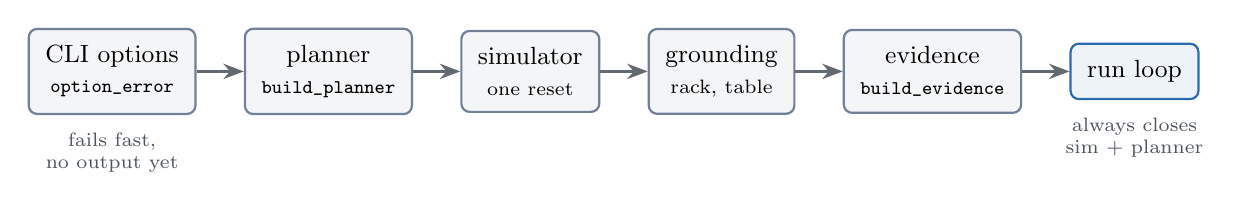
\begin{tikzpicture}[node distance=4mm and 6mm]
  \node[box=stone] (o) {CLI options\\\scriptsize \code{option_error}};
  \node[box=stone,right=of o] (p) {planner\\\scriptsize \code{build_planner}};
  \node[box=stone,right=of p] (s) {simulator\\\scriptsize one reset};
  \node[box=stone,right=of s] (g) {grounding\\\scriptsize rack, table};
  \node[box=stone,right=of g] (e) {evidence\\\scriptsize \code{build_evidence}};
  \node[box=sky,right=of e] (r) {run loop};
  \draw[flow] (o)--(p); \draw[flow] (p)--(s); \draw[flow] (s)--(g); \draw[flow] (g)--(e); \draw[flow] (e)--(r);
  \node[lbl,below=1mm of o] {fails fast,\\no output yet};
  \node[lbl,below=1mm of r] {always closes\\sim + planner};
\end{tikzpicture}
\caption{Episode start-up order.}
\end{figure}

\subsection{Choosing the coach}
\needspace{12\baselineskip}
\begin{lstlisting}[firstnumber=92,caption={\srcref{harness/runtime/assembly.py:92}}]
def build_planner(kind, run_settings, *, planner_settings=None, pixel_grounding=False):
    """Return the planner for ``kind`` ("anthropic" or "scripted")."""
    if kind == "anthropic":
        return AnthropicPlanner(planner_settings, require_pixel_grounding=pixel_grounding)
    if kind != "scripted":
        raise ValueError("unsupported_planner")
    if run_settings.handoff is not None:
        return HandoffPlanner(run_settings.recipe, run_settings.handoff)
    return GraspRetryPlanner(run_settings.recipe)
\end{lstlisting}

\begin{changeit}
\textbf{New planner?} Write a class with \code{select(context) -> PlannerSelection}
(protocol in \code{harness/planner/base.py}) and add one branch here. The loop never needs to know
which planner it talks to.
\end{changeit}

\subsection{What a move card looks like}
\needspace{12\baselineskip}
\begin{lstlisting}[numbers=none,caption={\srcref{harness/skills/schemas.py:84} (abridged)}]
class SkillCommand(Model):
    action: SkillType                                  # one of the six skills
    arm: Literal["left", "right", "both", "auto"] = "auto"
    parameters: VLAParameters | MoveParameters | ...   # typed per skill
    stop: StrictStr | None = None                      # a predicate name, for vla_act
    reason: Annotated[StrictStr, Field(max_length=1000)] | None = None
\end{lstlisting}
Every card is validated twice: once when Opus answers (\code{response_parser.py}) and again inside
the executor. Unknown fields are rejected (\code{extra="forbid"}).

\subsection{The heart of the turn loop}
\needspace{12\baselineskip}
\begin{lstlisting}[numbers=none,caption={\srcref{harness/runtime/orchestrator.py:259} (abridged)}]
selection = self.planner.select(PlannerContext(turn, observation.copy(), predicates, ...))
command = SkillCommand.model_validate(selection.command.model_dump())
self.log({**base, "event_type": "planner_selection", ...})   # intent logged before motion

prepared, rejection_code = self._prepare_anchor(command, observation, camera_to_avoid)
if rejection_code is not None:          # bad grounding: give feedback, try again
    grounding_feedback, grounding_camera_to_avoid = reselection_feedback(command, n)
    continue

previous = executor.execute(command)    # the only place robot motion starts
failure = turn_failure(command, previous, post)
flags = recovery_flags(previous)        # known, recoverable failure types
\end{lstlisting}

\subsection{Playing a policy chunk}
\needspace{12\baselineskip}
\begin{lstlisting}[numbers=none,caption={\srcref{harness/skills/vla_act.py:62} (abridged)}]
while context.chunks < (success_chunk_limit or configured_chunk_limit):
    observation = env.observe()
    context.chunks += 1                          # failed requests also count
    actions = np.asarray(context.vla.infer(observation, parameters.chunk_size))
    # ... validate the whole chunk (shape 14, finite) before ANY motion ...
    for action in actions:
        stopped = predicate_stop()               # e.g. mug_lifted reached?
        if stopped:
            return stopped                       # remaining actions are discarded
        context.observation = env.step(action)
        if overlap_check():                      # the two arms touched
            return "arm_overlap_detected"
\end{lstlisting}

% ================================================================ 12
\section{Cookbook: I want to\ldots}

\begin{center}
\small
\begin{tabularx}{\textwidth}{>{\raggedright\arraybackslash}p{4.6cm}>{\raggedright\arraybackslash}X}
\toprule
I want to\ldots & Do this \\
\midrule
change what Opus is told & Edit \code{harness/prompts/common.md} or \code{full_task.md}. The prompt hash in \code{manifest.json} changes, so old and new runs stay distinguishable. \\
change budgets or chunk sizes & Edit the YAML in \code{configs/} (\code{budget:}, \code{anthropic.vla:}). No code change. \\
get feedback after more chunks & \code{anthropic.planner_feedback_chunks} (1--4) in the config. \\
use another segmentation model & Write a factory returning an object with \code{detect(images, *, observation_sequence)} and pass \opt{perception-factory pkg.module:factory}. \\
add a new planner & Implement \code{select}, register it in \code{assembly.build_planner}, add a CLI choice in \code{run_skills.build_parser}. \\
use another policy backend & Implement \code{reset_history()} and \code{infer(observation, n)} (\code{harness/vla/base.py}). \\
add a checklist question & Add the name to \code{PREDICATE_NAMES} (\code{predicates/registry.py}) and teach a provider to answer it; return \code{null} when unsure. \\
tune lift or mask thresholds & See the green box in Section 8. \\
add a new skill & Rare and risky: add a \code{SkillType}, parameter model, implementation, registry entry, tool description, and tests. Talk to the team first. \\
ask Opus a new perception question & Build it with \code{harness/perception/vision_request.py} and add a prompt file. \\
\bottomrule
\end{tabularx}
\end{center}

\begin{careful}
Do not send simulator-only facts to Opus, do not remove the release check, and do not let a failed
command be retried automatically. These rules are what make results trustworthy.
\end{careful}

% ================================================================ 13
\section{Configuration files}

A config is a YAML file read into \code{RunSettings} (\srcref{harness/runtime/settings.py}).
This is the richest preset, \code{configs/skill_runtime_opus_full_task_rgbd_table_lift.yaml}:

\needspace{12\baselineskip}
\begin{lstlisting}[style=yaml,caption={An annotated full-task configuration}]

record_video: true              # writes episode.mp4 into the run folder
max_turns: 100                  # planner turns
perception:
  rgbd_enabled: true            # capture depth + calibration
  opus_rack_grounding: true     # ground the rack once at reset
  opus_mug_lift_grounding: true # table-plane lift evidence
  rack_grounding_camera: right_camera
  rack_prompt_profile: explore_mug_rack
budget:
  max_skill_calls: 100
  max_analytic_ticks: 2500
  max_policy_actions: 800
  max_vla_chunks: 100
anthropic:
  model: claude-opus-5          # explicit; there is no fallback model
  task_scope: full_task         # grasp -> handoff -> hang
  planner_feedback_chunks: 1    # Opus looks again after every chunk
  vla: {max_chunks: 32, chunk_size: 8, max_policy_actions: 768}
\end{lstlisting}

\begin{center}
\small
\begin{tabularx}{\textwidth}{>{\raggedright\arraybackslash}p{7.2cm}>{\raggedright\arraybackslash}X}
\toprule
Config family & Use \\
\midrule
\code{skill_runtime.yaml} & small scripted acquisition (no Opus); good first run \\
\code{skill_runtime_rgbd.yaml} & same, with depth for a detector \\
\code{skill_runtime_left_transfer.yaml},\newline \code{skill_runtime_full_handoff.yaml} & scripted handoff experiments \\
\code{skill_runtime_opus_*.yaml} & Opus planner, from acquisition to full task \\
\code{explore_*.yaml} & campaigns for \code{run_exploration.py} \\
\code{evaluation.yaml} & frozen evaluation seeds for \code{run_evaluation.py} \\
\code{harness.yaml}, \code{baseline.yaml} & legacy pass-through hook for the baseline \\
\bottomrule
\end{tabularx}
\end{center}

% ================================================================ 14
\section{How we work: the development ladder}
\label{sec:ladder}

\begin{eli5}
Learning to swim, you start in the bathtub, then the shallow end, and only then the deep end.
We test changes the same way. Each rung up the ladder costs more time and money, so only climb
when the rung below passes.
\end{eli5}

\begin{figure}[H]
\centering
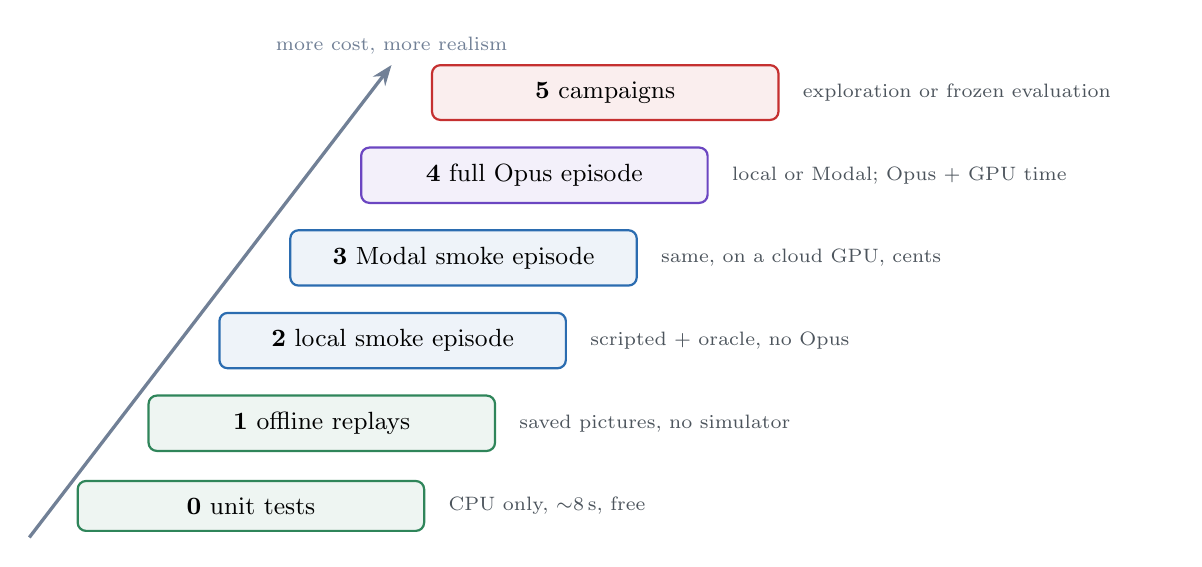
\begin{tikzpicture}[every node/.style={font=\small}]
  \foreach \y/\c/\t/\d in {0/leaf/{\textbf{0} unit tests}/{CPU only, $\sim$8\,s, free},
                          1/leaf/{\textbf{1} offline replays}/{saved pictures, no simulator},
                          2/sky/{\textbf{2} local smoke episode}/{scripted + oracle, no Opus},
                          3/sky/{\textbf{3} Modal smoke episode}/{same, on a cloud GPU, cents},
                          4/grape/{\textbf{4} full Opus episode}/{local or Modal; Opus + GPU time},
                          5/rose/{\textbf{5} campaigns}/{exploration or frozen evaluation}} {
    \node[box=\c,minimum width=4.4cm,anchor=west] at (\y*0.9,\y*1.05) {\t};
    \node[lbl,anchor=west,text width=4.6cm,align=left] at (\y*0.9+4.6,\y*1.05) {\d};
  }
  \draw[->,very thick,stone] (-0.6,-0.4) -- (4.0,5.6) node[above,font=\scriptsize,text=stone] {more cost, more realism};
\end{tikzpicture}
\caption{Climb one rung at a time. Most bugs are cheapest to find on rungs 0--2.}
\end{figure}

\begin{center}
\small
\begin{tabularx}{\textwidth}{>{\raggedright\arraybackslash}p{3.0cm}>{\raggedright\arraybackslash}X}
\toprule
Rung & Command (from the repository root) \\
\midrule
0 tests & \texttt{python -m unittest discover -s tests -q} \\
1 replays & \texttt{python -m development.replays.perception \opt{help}} (and the other tools in \code{development/replays/}) \\
2 local smoke & \texttt{python run\_skills.py \opt{config} configs/skill\_runtime.yaml \opt{development-oracle} \opt{output} data/runs/smoke\_01} \\
3 Modal smoke & \texttt{modal run modal\_apps/simulator.py::episode \opt{config} configs/skill\_runtime.yaml \opt{development-oracle} \opt{output} data/runs/modal\_smoke\_01} \\
4 full episode & Section~\ref{sec:runlocal} (local) or Section~\ref{sec:runmodal} (Modal) \\
5 campaigns & \code{run_exploration.py}, \code{run_evaluation.py} (local only for now) \\
\bottomrule
\end{tabularx}
\end{center}

\begin{keyidea}
The rung-2 smoke run is \emph{expected} to stop with \code{"outcome": "step_budget"}: the scripted
recipe gives its first move 1000 physics ticks, and the planned path needs a little more. It still
proves the simulator, CuRobo and logging work. Same result on Modal $=$ the remote runner behaves
like the local one.
\end{keyidea}

% ================================================================ 15
\section{Setting up and running}

There are two ways to run an episode. Both use the same command-line options and produce the same
run folder; only \emph{where the simulator runs} changes.

\begin{figure}[H]
\centering
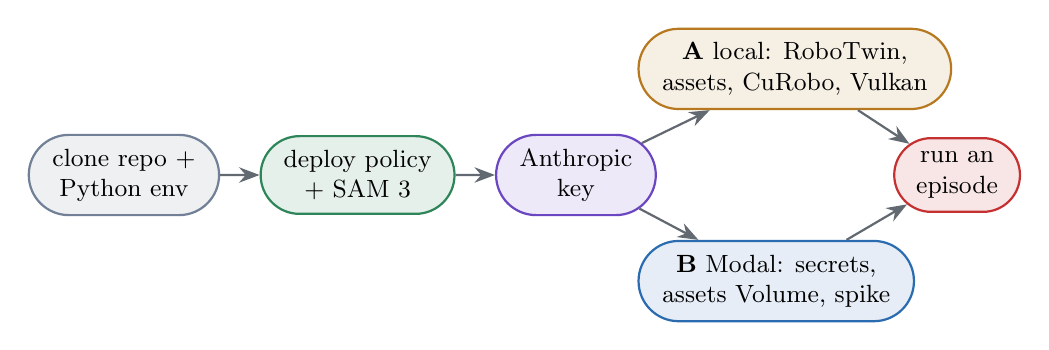
\begin{tikzpicture}[node distance=4mm and 5mm,every node/.style={font=\small}]
  \node[pill=stone] (c1) {clone repo +\\Python env};
  \node[pill=leaf,right=of c1] (c2) {deploy policy\\+ SAM 3};
  \node[pill=grape,right=of c2] (c3) {Anthropic\\key};
  \node[pill=sun,above right=3mm and 8mm of c3] (a1) {\textbf{A} local: RoboTwin,\\assets, CuRobo, Vulkan};
  \node[pill=sky,below right=3mm and 8mm of c3] (b1) {\textbf{B} Modal: secrets,\\assets Volume, spike};
  \node[pill=rose,right=30mm of c3] (run) {run an\\episode};
  \draw[flow] (c1)--(c2); \draw[flow] (c2)--(c3); \draw[flow] (c3)--(a1); \draw[flow] (c3)--(b1);
  \draw[flow] (a1)--(run); \draw[flow] (b1)--(run);
\end{tikzpicture}
\caption{Common steps, then path A (your own NVIDIA GPU) or path B (rented Modal GPU). You can set up both.}
\end{figure}

\begin{center}
\small
\begin{tabularx}{\textwidth}{>{\raggedright\arraybackslash}p{3.2cm}>{\raggedright\arraybackslash}X>{\raggedright\arraybackslash}X}
\toprule
 & \textbf{A: local} & \textbf{B: Modal} \\
\midrule
You need & Linux, NVIDIA GPU with Vulkan, $\sim$10\,GB disk & any machine with Python and a Modal account \\
Speed & pictures $\sim$0.8\,s each on a 4\,GB laptop GPU & pictures $\sim$0.11\,s each on an L4 \\
Costs & electricity; Opus + policy calls & GPU time ($\sim$\$0.6--0.8/h) + Opus + policy calls \\
Good for & debugging with the simulator in reach & long or many runs, small laptops \\
\bottomrule
\end{tabularx}
\end{center}

\subsection{Common steps (both paths)}
\begin{cmd}
git clone <this repository> \&\& cd Agent-Aware-Vision-Language-Action-Model\\
conda create -n robotwin python=3.10 -y \&\& conda activate robotwin\\
python -m pip install -r requirements/sim.txt -r requirements/planner.txt \textquotesingle{}modal>=1,<2\textquotesingle{}\\[4pt]
modal setup \ \ \ \ \ \ \ \ \ \ \ \ \ \ \ \ \ \ \ \ \ \ \ \ \ \ \ \ \ \ \# log in to Modal once\\
modal deploy modal\_apps/policy.py \ \ \ \ \ \ \ \ \ \# frozen Neotix policy (T4)\\[4pt]
\# SAM 3: first request access at huggingface.co/facebook/sam3 and wait for approval\\
modal secret create huggingface HF\_TOKEN=hf\_... \ \ \# add -{}-force to replace it\\
modal deploy modal\_apps/sam3.py\\
modal run modal\_apps/sam3.py \ \ \ \ \ \ \ \ \ \ \ \ \ \ \# smoke test: prints "SAM 3 ... ready"\\[4pt]
\# Anthropic key, kept inside the conda env (never in git)\\
conda env config vars set ANTHROPIC\_API\_KEY=sk-ant-...\\
conda deactivate \&\& conda activate robotwin
\end{cmd}
Path B only needs the Python packages (no simulator, no GPU) on your machine; the \code{robotwin}
environment above works for both.

\subsection{Path A: run on your own GPU}
\label{sec:runlocal}

\textbf{A1. RoboTwin and its assets.} Run from the repository root. The task only needs the
\code{embodiments} and \code{objects} bundles ($\sim$4\,GB); the 11\,GB background textures are
only used with random backgrounds, which \code{demo_clean} turns off.
\begin{cmd}
git clone https://github.com/RoboTwin-Platform/RoboTwin.git RoboTwin\\
git -C RoboTwin checkout ea8b21121ebb3cd201ff5b3fe361944ac94eda3f\\
git -C RoboTwin apply ../patches/robotwin-renderer.patch\\
cd RoboTwin/assets\\
HF\_HUB\_DISABLE\_XET=1 python -c "from huggingface\_hub import snapshot\_download as get; \textbackslash\\
\hspace*{1.5em}get(\textquotesingle{}TianxingChen/RoboTwin2.0\textquotesingle{}, repo\_type=\textquotesingle{}dataset\textquotesingle{}, local\_dir=\textquotesingle{}.\textquotesingle{}, \textbackslash\\
\hspace*{1.5em}allow\_patterns=[\textquotesingle{}embodiments.zip\textquotesingle{}, \textquotesingle{}objects.zip\textquotesingle{}])"\\
unzip -q embodiments.zip \&\& rm embodiments.zip\\
unzip -q objects.zip \&\& rm objects.zip \&\& rm -rf \_\_MACOSX\\
cd .. \&\& python scripts/update\_embodiment\_config\_path.py \&\& cd ..
\end{cmd}

\textbf{A2. CuRobo (the motion planner).} It compiles GPU code, so the compiler settings are stored
in the conda environment once. CUDA~12.1's \code{nvcc} refuses gcc newer than 12; set
\code{TORCH_CUDA_ARCH_LIST} to your GPU (8.6 for an RTX 2050/30-series).
\begin{cmd}
git clone -{}-branch v0.7.8 https://github.com/NVlabs/curobo.git RoboTwin/envs/curobo\\
git -C RoboTwin/envs/curobo checkout d64c4b005459db10c5dd867d8b30a87d5bda9bdb\\
conda env config vars set CUDA\_HOME="\$CONDA\_PREFIX" CC=/usr/bin/gcc-12 \textbackslash\\
\hspace*{1.5em}CXX=/usr/bin/g++-12 CUDAHOSTCXX=/usr/bin/g++-12 \textbackslash\\
\hspace*{1.5em}NVCC\_PREPEND\_FLAGS="-ccbin /usr/bin/g++-12" TORCH\_CUDA\_ARCH\_LIST=8.6\\
conda deactivate \&\& conda activate robotwin\\
python -m pip install -e RoboTwin/envs/curobo -{}-no-build-isolation \ \ \# 5--15 minutes\\
python -m pip install warp-lang==1.12.0\\
python -c "import curobo; print(\textquotesingle{}curobo ok\textquotesingle{})"
\end{cmd}

\textbf{A3. Vulkan: use only the NVIDIA driver.} Laptops with a second (Intel) GPU can freeze the
renderer otherwise.
\begin{cmd}
conda env config vars set VK\_DRIVER\_FILES=/usr/share/vulkan/icd.d/nvidia\_icd.json \textbackslash\\
\hspace*{1.5em}VK\_ICD\_FILENAMES=/usr/share/vulkan/icd.d/nvidia\_icd.json\\
conda deactivate \&\& conda activate robotwin\\
vulkaninfo -{}-summary | grep deviceName \ \ \ \# should list only your NVIDIA GPU
\end{cmd}

\textbf{A4. Climb the ladder.} Tests, then the smoke run, then a full episode with a time limit.
\code{timeout -s INT} sends the same signal as Ctrl+C, so the run still writes \code{summary.json}
and its video.
\begin{cmd}
python -m unittest discover -s tests -q\\
python run\_skills.py -{}-config configs/skill\_runtime.yaml \textbackslash\\
\hspace*{1.5em}-{}-development-oracle -{}-output data/runs/smoke\_01\\[4pt]
timeout -s INT 75m python run\_skills.py \textbackslash\\
\hspace*{1.5em}-{}-config configs/skill\_runtime\_opus\_full\_task\_rgbd\_table\_lift.yaml \textbackslash\\
\hspace*{1.5em}-{}-planner anthropic \textbackslash\\
\hspace*{1.5em}-{}-perception-factory harness.perception.modal\_sam3:create\_detector \textbackslash\\
\hspace*{1.5em}-{}-output data/runs/full\_task\_01
\end{cmd}

\subsection{Path B: run on Modal}
\label{sec:runmodal}

\begin{eli5}
Instead of using your own computer's graphics card, you \textbf{rent} a stronger one for as long as
the episode lasts. Modal starts a fresh, clean computer (a \emph{container}) for every episode,
runs exactly the same \code{run_skills.py} there, keeps the results in a cloud folder (a
\emph{Volume}), and copies them back to your \code{data/runs/} folder at the end.
\end{eli5}

\begin{figure}[H]
\centering
\begin{tikzpicture}[every node/.style={font=\small}]
  \node[box=stone,text width=3.0cm] (lap) at (0,0) {\faLaptop\ your machine\\\scriptsize \code{modal run ...::episode}\\\scriptsize checks options first};
  \node[box=sky,text width=4.0cm] (ep) at (6.2,0) {\textbf{episode container (L4)}\\\scriptsize \code{run_skills.py} + RoboTwin\\\scriptsize + CuRobo, fresh every run};
  \node[box=leaf,text width=2.4cm] (pol) at (11.6,1.3) {policy (T4)};
  \node[box=leaf,text width=2.4cm] (sam) at (11.6,0) {SAM 3 (T4)};
  \node[box=grape,text width=2.4cm] (ant) at (11.6,-1.3) {Opus (API)};
  \node[box=sun,text width=3.0cm] (va) at (4.4,-2.4) {Volume\\\code{robotwin-assets}};
  \node[box=sun,text width=3.0cm] (vr) at (8.0,-2.4) {Volume\\\code{robotwin-runs}};
  \draw[flow] (lap.north east) -- node[lbl,above,sloped]{args + config} (ep.north west);
  \draw[flow] (vr.south) -- ++(0,-0.45) -| node[lbl,below,pos=0.25]{results copied back to \code{data/runs/}} (lap.south);
  \draw[dflow] (ep) -- (pol); \draw[dflow] (ep) -- (sam); \draw[dflow] (ep) -- node[lbl,above,sloped,pos=0.6]{secret key} (ant);
  \draw[flow] (va) -- node[lbl,left]{read} (ep); \draw[flow] (ep) -- node[lbl,right]{write} (vr);
  \begin{scope}[on background layer]
    \node[zone=leaf,fit=(ep)(pol)(sam)(va)(vr),label={[font=\small\bfseries,text=leaf]above:\faCloud\ Modal}] {};
  \end{scope}
\end{tikzpicture}
\caption{An episode on Modal (\srcref{modal_apps/simulator.py}). Policy and SAM~3 calls stay inside Modal.}
\end{figure}

\textbf{B1. One-time setup.} The first command builds the cloud image (RoboTwin, CuRobo for
T4/A10G/L4/A100, the same patches as path~A; about 20--40 minutes once, then cached) and copies the
assets into a Volume. The spike is optional: it measures a GPU and saves a camera picture to
\code{data/modal_spike/}.
\begin{cmd}
\# needed by every run of simulator.py, even the spike\\
modal secret create anthropic ANTHROPIC\_API\_KEY=sk-ant-...\\
modal run modal\_apps/simulator.py::download\_assets \ \ \ \ \ \ \ \ \# CPU only, once\\
modal run modal\_apps/simulator.py::spike \ \ \ \ \ \ \ \ \ \ \ \ \ \ \ \ \ \ \# optional: test the L4\\
SIM\_GPU=T4 modal run modal\_apps/simulator.py::spike \ \ \ \ \ \ \# optional: test a T4
\end{cmd}

\textbf{B2. Run episodes.} Use the normal \code{run_skills.py} options after \code{::episode}.
Two extra options belong to the launcher: \opt{time-limit-minutes} (default 90, at most 210) and
\opt{skip-observations} (leave the per-step pictures on the Volume).
\begin{cmd}
\# rung 3: cheap smoke run (no Opus calls)\\
modal run modal\_apps/simulator.py::episode \textbackslash\\
\hspace*{1.5em}-{}-config configs/skill\_runtime.yaml -{}-development-oracle \textbackslash\\
\hspace*{1.5em}-{}-output data/runs/modal\_smoke\_01 -{}-time-limit-minutes 15\\[4pt]
\# rung 4: the full task\\
modal run modal\_apps/simulator.py::episode \textbackslash\\
\hspace*{1.5em}-{}-config configs/skill\_runtime\_opus\_full\_task\_rgbd\_table\_lift.yaml \textbackslash\\
\hspace*{1.5em}-{}-planner anthropic \textbackslash\\
\hspace*{1.5em}-{}-perception-factory harness.perception.modal\_sam3:create\_detector \textbackslash\\
\hspace*{1.5em}-{}-output data/runs/modal\_full\_01 -{}-time-limit-minutes 75
\end{cmd}

\textbf{B3. Housekeeping.}
\begin{cmd}
modal volume ls robotwin-runs \ \ \ \ \ \ \ \ \ \ \ \ \ \ \ \ \ \ \ \ \ \ \ \ \ \ \# list remote runs\\
modal volume get robotwin-runs <run\_id> data/runs/ \ \ \ \ \# download a run again\\
modal volume rm -r robotwin-runs <run\_id> \ \ \ \ \ \ \ \ \ \ \ \ \# delete an old run
\end{cmd}

\begin{careful}
\begin{itemize}[leftmargin=*]
  \item \textbf{Keep the terminal open}: stopping \code{modal run} stops the episode. For a run that
        survives a closed laptop use \texttt{modal run \opt{detach} ...}, then fetch the results with
        \code{modal volume get}.
  \item \textbf{One Modal episode at a time} for now: the policy worker keeps one shared
        observation history, so parallel episodes would mix their memories.
  \item Frozen evaluation (\opt{evaluation-manifest}) is refused on Modal; it stays local for now.
\end{itemize}
\end{careful}

\subsection{Running cheaply}
\begin{center}
\small
\begin{tabularx}{\textwidth}{>{\raggedright\arraybackslash}p{5.0cm}X}
\toprule
Trick & Why it saves \\
\midrule
Stay low on the ladder & tests and replays are free; most mistakes show up there \\
Scripted planner + \opt{development-oracle} & no Opus calls at all \\
\opt{time-limit-minutes} (Modal) or \code{timeout -s INT} (local) & a stuck run cannot burn hours \\
\code{SIM_GPU=T4} & cheaper per hour than the L4; pictures $\sim$3$\times$ slower, a full episode only $\sim$1 minute longer \\
\opt{skip-observations} & smaller downloads; pictures stay on the Volume \\
A copied config with smaller \code{max_turns} / \code{anthropic.max_calls} & caps Opus turns \\
Delete old runs from \code{robotwin-runs} & Volumes keep (and bill for) what you store \\
\bottomrule
\end{tabularx}
\end{center}
Rough cost of one full Modal episode ($\sim$30 minutes, mostly waiting for Opus): about \$0.30 on a T4
or \$0.40 on an L4 of simulator GPU time, plus Opus tokens and policy time. Prices are approximate;
check Modal's pricing page and dashboard.

\subsection{Measured speed}
\label{sec:speed}
Same seed, same steps, measured with the spike (\code{data/modal_spike/}):
\begin{center}
\small
\begin{tabular}{lrrrr}
\toprule
 & laptop RTX 2050 & T4 & A10G & \textbf{L4} \\
\midrule
three RGB-D pictures & 800\,ms & 344\,ms & 153\,ms & \textbf{110\,ms} \\
CuRobo plan & 322\,ms & 88\,ms & 73\,ms & 86\,ms \\
physics step & 0.09\,ms & 0.01\,ms & 0.01\,ms & 0.01\,ms \\
reset (once, cold) & 27\,s & 49\,s & 33\,s & 66\,s \\
\bottomrule
\end{tabular}
\end{center}
All three cloud GPUs draw the same picture as the laptop (mean difference 0.03 out of 255), so the
policy sees the same thing wherever the episode runs. L4 is the default; T4 is the budget choice.

\subsection{When something goes wrong}
\label{sec:trouble}
\begin{center}
\small
\begin{tabularx}{\textwidth}{>{\raggedright\arraybackslash}p{5.2cm}X}
\toprule
You see\ldots & Do this \\
\midrule
\code{Permission denied} under \code{/run/media/...} while downloading & \code{HF_HOME} points at an unmounted drive. Set it to \code{\$HOME/.cache/huggingface} or mount the drive. \\
\code{Not enough free disk space} & Download only \code{embodiments} and \code{objects} (A1); \code{conda clean -a} frees several GB. \\
\code{unsupported GNU version! gcc versions later than 12} & Set the compiler variables in A2 and reactivate the environment. \\
CuRobo ended up in \code{RoboTwin/RoboTwin/envs/} & You cloned from inside \code{RoboTwin/}; run the clone from the repository root. \\
Episode freezes, GPU at 0\,\%, log files stop changing & Renderer hang: apply A3, stop with Ctrl+C, rerun with a time limit. \\
\code{missing pytorch3d} at start-up & Harmless message from RoboTwin. \\
Smoke run ends with \code{step_budget} & Expected (Section~\ref{sec:ladder}). \\
SAM~3: \code{GatedRepoError ... not in the authorized list} & Your Hugging Face account is not approved yet, or the token is from another account; replace the secret with \opt{force}. \\
Modal \code{ImageBuildError} & Run \code{modal image logs <id>} with the \emph{newest} id from the error box. \\
\texttt{... already exists; choose a new \opt{output}} & Every run needs a new output folder. \\
\bottomrule
\end{tabularx}
\end{center}

\subsection{What you get after a run}
\begin{figure}[H]
\centering
\begin{forest}
  for tree={font=\ttfamily\footnotesize,grow'=0,child anchor=west,parent anchor=south,anchor=west,inner ysep=1.5pt,s sep=1pt,
    calign=first,edge path={\noexpand\path [draw, \forestoption{edge}] (!u.south west) +(7.5pt,0) |- node[fill,inner sep=1.25pt] {} (.child anchor)\forestoption{edge label};},
    before typesetting nodes={if n=1{insert before={[,phantom]}}{}},fit=band,before computing xy={l=15pt}}
  [data/runs/full\_task\_01/
    [manifest.json \quad{\rmfamily\color{stone} settings, seed, prompt hash}]
    [assessments.jsonl \quad{\rmfamily\color{stone} every planner choice and turn result}]
    [skill\_events.jsonl \quad{\rmfamily\color{stone} every action, tick and check}]
    [simulator\_timing.jsonl \quad{\rmfamily\color{stone} how long RoboTwin took}]
    [oracle.jsonl \quad{\rmfamily\color{stone} private evidence (oracle mode only)}]
    [observations/ \quad{\rmfamily\color{stone} saved pictures + depth (.npz)}]
    [episode.mp4 \quad{\rmfamily\color{stone} video when \texttt{record\_video: true}}]
    [summary.json \quad{\rmfamily\color{stone} outcome, counts, timings}]
    [candidate\_catalog.json \quad{\rmfamily\color{stone} memory ideas to review (never auto-used)}]
  ]
\end{forest}
\caption{Run artifacts. Exit code 0 means a success outcome such as \code{acquisition_confirmed} or \code{task_success}.}
\end{figure}

\subsection{Other ways to run}
\begin{figure}[H]
\centering
\begin{tikzpicture}[node distance=5mm and 20mm]
  \node[box=sun] (t1) {\textbf{Terminal 1}\\\scriptsize\code{run_inference_chunked.py sim}\\\scriptsize RoboTwin HTTP server :8110};
  \node[box=sky,right=of t1] (t2) {\textbf{Terminal 2}\\\scriptsize\code{run_inference_chunked.py policy}\\\scriptsize episode loop};
  \node[box=leaf,right=14mm of t2] (m) {\faCloud\ Modal\\policy};
  \draw[<->,thick] (t1) -- node[lbl,above]{actions} node[lbl,below]{observations} (t2);
  \draw[<->,thick,dashed] (t2) -- node[lbl,above]{chunks} (m);
\end{tikzpicture}
\caption{The baseline: the frozen policy alone, no coach. Used to compare against.}
\end{figure}

\begin{itemize}
  \item \textbf{One episode on Modal} (\texttt{modal run modal\_apps/simulator.py::episode}) takes the same options as \code{run_skills.py}; see Section~\ref{sec:runmodal}.
  \item \textbf{Exploration} (\code{run_exploration.py}) runs many episodes, each in a new process, and collects memory \emph{candidates}. It currently requires \opt{development-oracle} and runs locally.
  \item \textbf{Evaluation} (\code{run_evaluation.py freeze}/\code{run}) locks seeds, code hashes and memory, so results cannot be accidentally tuned on the test seeds.
  \item \textbf{Offline tools} live in \code{development/}, for example\\\texttt{python -m development.replays.perception \opt{help}}.\\ Most need no simulator.
\end{itemize}

% ================================================================ 15
\section{Where things stand today}

\begin{center}
\small
\begin{tabularx}{\textwidth}{>{\raggedright\arraybackslash}p{4.4cm}lX}
\toprule
Part & State & Notes \\
\midrule
Baseline policy runner & \textcolor{leaf}{\faCheck\ works} & independent of the harness \\
Skill executor + six skills & \textcolor{leaf}{\faCheck\ works} & bounded, tested on CPU fakes \\
Scripted acquisition / handoff & \textcolor{leaf}{\faCheck\ works} & development-oracle evidence \\
Opus planner, full task & \textcolor{sun}{\faQuestion\ exploring} & phases succeed sometimes; not yet reliable hanging \\
Public RGB-D perception & \textcolor{sun}{\faQuestion\ exploring} & SAM 3 + Opus grounding; gaps return \code{null} \\
Evaluation with perception & \textcolor{rose}{\faTimes\ not yet} & needs a frozen detector/prompt contract \\
Simulator on Modal & \textcolor{leaf}{\faCheck\ works} & T4, A10G and L4 render the same pictures as the laptop \\
Single episodes on Modal & \textcolor{sun}{\faQuestion\ new} & \code{::episode} is built and tested offline; first live runs pending \\
Parallel runs, campaigns on Modal & \textcolor{rose}{\faTimes\ not yet} & needs one policy session per episode \\
Renderer freeze on two-GPU laptops & \textcolor{sun}{\faQuestion\ mitigated} & pin Vulkan to NVIDIA (Section~\ref{sec:trouble}) \\
Unit tests & \textcolor{leaf}{\faCheck\ 435 pass} & \code{python -m unittest discover -s tests} \\
\bottomrule
\end{tabularx}
\end{center}

\begin{careful}
\begin{itemize}[leftmargin=*]
  \item Success of one phase is \textbf{not} proof of reliable full-task hanging.
  \item RoboTwin's native success check is not the same as a verified handle-on-peg hang.
  \item Configs name the model \code{claude-opus-5}; check it is the model you intend to use.
  \item Checkpoints and provenance files recorded before the October 2026 restructure no longer match the current file layout; record new ones.
\end{itemize}
\end{careful}

% ================================================================ 16
\section{Testing and contributing}

\begin{itemize}
  \item \textbf{All tests run on CPU} with fake simulators, fake policies and fake Opus clients. No GPU or API key is needed.
  \item \textbf{Change behaviour, change a test.} New behaviour needs a test that shows it.
  \item \textbf{One subsystem per pull request}, with the contract change and a CPU or replay check.
  \item \textbf{Prompts are code.} Version a prompt change together with the parser/schema it serves.
  \item \textbf{Clean-code defaults} for agents and people are in \code{.agents/skills/clean-code/SKILL.md}.
\end{itemize}

\appendix
\section{Frequently asked questions}

\begin{description}[style=nextline,leftmargin=0pt,labelsep=0pt]
  \item[\color{sky}Why not let Opus control the joints directly?]
  Language models are not precise with numbers and cannot react within milliseconds. Opus judges the
  situation; deterministic code and the trained policy do the motion.
  \item[\color{sky}Why does an unknown answer stop the robot from opening its hand?]
  Opening a hand that holds an unsupported mug drops it. Without proof, the safe choice is not to open.
  \item[\color{sky}What is the ``development oracle'' for?]
  Debugging. It uses simulator-only knowledge so we can test skills before perception is good enough.
  It is never shown to Opus and is not allowed in evaluation with perception.
  \item[\color{sky}Why is the policy called in short chunks?]
  So the coach can look again often. Long chunks are cheaper but react slower.
  \item[\color{sky}Where do I start reading code?]
  \code{run_skills.py}, then \code{harness/runtime/assembly.py}, then \code{harness/runtime/orchestrator.py}.
  \item[\color{sky}Why run episodes on Modal instead of my laptop?]
  A rented L4 draws the camera pictures about seven times faster than a 4\,GB laptop GPU, has no
  memory squeeze, and avoids two-GPU laptop driver trouble. It costs GPU time, so use the ladder.
  \item[\color{sky}Do I need RoboTwin on my machine to use Modal?]
  No. The simulator lives in the cloud image. Your machine only needs the Python packages to check
  the options and to talk to Modal.
  \item[\color{sky}Does running on Modal change the results?]
  The pictures match the laptop's almost exactly (0.03 out of 255 on average). Still treat local
  and Modal runs as separate conditions when you compare numbers carefully.
  \item[\color{sky}Why only one Modal episode at a time?]
  The deployed policy remembers recent pictures for the episode it is serving. Two episodes at once
  would share that memory. Giving each episode its own policy session is the next step.
\end{description}

\end{document}
